% olmo_lineage_revised.tex
% Development-tier synthesis of how post-training changes J-space causal use
% across the OLMo 32B lineage. All numerical claims cite registered evidence
% IDs from the J-space campaign. This is not a frozen Phase 4 claim record.
\documentclass[11pt]{article}

\usepackage[letterpaper,margin=0.76in,headheight=15pt]{geometry}
\usepackage[T1]{fontenc}
\usepackage[utf8]{inputenc}
\usepackage{lmodern}
\usepackage{microtype}
\usepackage{amsmath,amssymb,mathtools}
\usepackage{booktabs,tabularx,array,multirow}
\usepackage{enumitem}
\usepackage{xcolor}
\usepackage{graphicx}
\usepackage{caption}
\usepackage{float}
\usepackage[most]{tcolorbox}
\usepackage{listings}
\usepackage{fancyhdr}
\usepackage{titlesec}
\usepackage{hyperref}
\usepackage[nameinlink,noabbrev]{cleveref}
\usepackage{xurl}
\usepackage{placeins}

\definecolor{ink}{HTML}{18222D}
\definecolor{slate}{HTML}{4D5B6A}
\definecolor{violet}{HTML}{6D5BD0}
\definecolor{violetdark}{HTML}{4E3DA8}
\definecolor{teal}{HTML}{0C7C86}
\definecolor{bluegray}{HTML}{EAF0F5}
\definecolor{lavender}{HTML}{F0EDFF}
\definecolor{amber}{HTML}{A86500}
\definecolor{amberbg}{HTML}{FFF5DD}
\definecolor{redish}{HTML}{A43842}
\definecolor{redbg}{HTML}{FFF0F1}
\definecolor{greenish}{HTML}{277A55}
\definecolor{greenbg}{HTML}{EAF7F0}

\hypersetup{
  colorlinks=true, linkcolor=violetdark, citecolor=teal, urlcolor=teal,
  pdftitle={Post-Training Reorganizes Causal Use of J-Space in the OLMo 32B Lineage},
  pdfauthor={Karl Burtram},
  pdfsubject={Development-tier J-space synthesis across OLMo base, Think, and Instruct checkpoints}
}

\pagestyle{fancy}
\fancyhf{}
\lhead{J-space development synthesis}
\rhead{OLMo 32B post-training lineage}
\cfoot{\thepage}
\renewcommand{\headrulewidth}{0.4pt}

\titleformat{\section}{\Large\bfseries\color{ink}}{\thesection}{0.7em}{}
\titleformat{\subsection}{\large\bfseries\color{violetdark}}{\thesubsection}{0.65em}{}
\titleformat{\subsubsection}{\normalsize\bfseries\color{teal}}{\thesubsubsection}{0.55em}{}

\setlist[itemize]{topsep=3pt,itemsep=2.5pt,parsep=1pt,leftmargin=1.45em}
\setlist[enumerate]{topsep=3pt,itemsep=2.5pt,parsep=1pt,leftmargin=1.65em}
\setlength{\parindent}{0pt}
\setlength{\parskip}{5.3pt}
\setlength{\emergencystretch}{2.5em}

\newcommand{\eid}[1]{{\footnotesize\nolinkurl{[#1]}}}
\newcommand{\ci}[2]{{[#1,\,#2]}}
\newcommand{\SJ}{S_J}
\newcommand{\dJ}{\Delta_J}
\newcommand{\dC}{\Delta_C}
\newcommand{\BankS}{\text{Bank S}}
\newcommand{\BankF}{\text{Bank F}}

\newtcolorbox{takeawaybox}[1][]{enhanced, breakable, colback=lavender,
  colframe=violet, boxrule=0.8pt, arc=2mm,
  left=2.5mm,right=2.5mm,top=1.8mm,bottom=1.8mm,
  fonttitle=\bfseries, title={Key takeaway}, #1}
\newtcolorbox{statusbox}[1][]{enhanced, breakable, colback=bluegray,
  colframe=slate, boxrule=0.7pt, arc=2mm,
  left=2.5mm,right=2.5mm,top=1.8mm,bottom=1.8mm,
  fonttitle=\bfseries, title={Evidence status}, #1}
\newtcolorbox{pitfallbox}[1][]{enhanced, breakable, colback=amberbg,
  colframe=amber, boxrule=0.7pt, arc=2mm,
  left=2.5mm,right=2.5mm,top=1.8mm,bottom=1.8mm,
  fonttitle=\bfseries, title={Interpretation trap}, #1}
\newtcolorbox{resultbox}[1][]{enhanced, breakable, colback=greenbg,
  colframe=greenish, boxrule=0.7pt, arc=2mm,
  left=2.5mm,right=2.5mm,top=1.8mm,bottom=1.8mm,
  fonttitle=\bfseries, title={Current synthesis}, #1}
\newtcolorbox{warningbox}[1][]{enhanced, breakable, colback=redbg,
  colframe=redish, boxrule=0.7pt, arc=2mm,
  left=2.5mm,right=2.5mm,top=1.8mm,bottom=1.8mm,
  fonttitle=\bfseries, title={Validity boundary}, #1}
\newtcolorbox{hypbox}[2][]{enhanced, breakable, colback=white,
  colframe=teal, boxrule=0.7pt, arc=2mm,
  left=2.5mm,right=2.5mm,top=1.8mm,bottom=1.8mm,
  fonttitle=\bfseries, title={#2}, #1}
\newtcolorbox{claimbox}[1][]{enhanced, breakable, colback=white,
  colframe=violetdark, boxrule=0.9pt, arc=2mm,
  left=3mm,right=3mm,top=2mm,bottom=2mm,
  fonttitle=\bfseries, title={Paper-facing claim ladder}, #1}

\graphicspath{{figures/}{./}}

\begin{document}
\pagenumbering{gobble}

\begin{titlepage}
\thispagestyle{empty}
\vspace*{0.48in}
{\color{violetdark}\rule{\textwidth}{2.2pt}}
\vspace{0.33in}

{\Huge\bfseries\color{ink} Post-Training Reorganizes Causal Use of J-Space\par}
\vspace{0.13in}
{\LARGE\bfseries\color{violetdark} Evidence from the OLMo 32B Base, Think, and Instruct Lineage\par}

\vspace{0.35in}
{\large Development-tier synthesis for the J-space campaign -- not a frozen Phase 4 claim record\par}

\vspace{0.46in}
\begin{tcolorbox}[enhanced,colback=lavender,colframe=violet,boxrule=1pt,arc=2mm,left=4mm,right=4mm,top=3mm,bottom=3mm]
\textbf{Central result.} On the tested in-context Bank-S tasks, the OLMo base
checkpoint shows no span-safe J-specific dependence. The effect appears by the
first observed Think checkpoint, remains at OLMo-3.1 Think, and is absent at
the OLMo-3.1 Instruct sibling. The pattern survives a frozen base-lens frame
and exact common-support fact pairing. Measured J-space capacity, however,
changes little across the three post-trained checkpoints. The evidence therefore
points more strongly to \emph{training-dependent recruitment or routing of an
existing thin verbalizable channel} than to the creation of a larger J-space.
\end{tcolorbox}

\vspace{0.28in}
\begin{statusbox}[title={What this document does and does not claim}]
It asks how post-training changes J-space geometry, causal utilization, and
workspace-like organization. It does not identify the causal training stage,
prove that the Think objective created a new representation, or license the
phrase ``selective global workspace.'' Every OLMo lineage result is
\textbf{phase4-development}: known banks, development cohorts, no untouched
Phase 4 confirmatory outcome.
\end{statusbox}

\vfill
\begin{tabular}{@{}ll@{}}
Author: & Karl Burtram (J-space campaign notes)\\
Primary sources: & Phase 4 registry and report; frozen Phase 2/3 imports\\
Branch snapshot: & \texttt{interp\_jspace\_part2}, development state through 2026-08-01\\
Document version: & August 2026, full lineage rewrite\\
\end{tabular}

\vspace{0.22in}
{\small\color{slate}
The comparison to Qwen and Gemma is used as triangulation. The primary subject
is the OLMo training lineage: what changes along the observed Think path, what
returns toward the base regime at the Instruct sibling, and which measurements
remain stable while causal behavior moves.}

\end{titlepage}

\hypersetup{pageanchor=true}
\pagenumbering{roman}
\tableofcontents
\clearpage
\pagenumbering{arabic}

%======================================================================
\section*{Executive synthesis}
\addcontentsline{toc}{section}{Executive synthesis}

The phrase ``J-space formation'' hides several distinct scientific questions.
Post-training might enlarge the verbalizable subspace, change its coordinates,
change which content enters it, change which downstream computations consume
it, or change only the model's behavioral strategy. The current OLMo evidence
separates these possibilities better than a single workspace score can.

\begin{takeawaybox}
The strongest supported reading is \textbf{causal recruitment without measured
capacity growth}. Across all four checkpoints --- now including the base model
under the parallel-phase symmetric estimator \eid{ol-capacity-joint-dev-v1}
--- sparse occupancy is unchanged (base$\to$3.0 Think occupancy difference
exactly 0) and centered excess variance moves by $+0.015$ percentage points
\ci{-0.012}{+0.043}. Yet Bank-S span-safe J-specific dependence is near zero
at base, negative at both Think checkpoints, and near zero at the Instruct
sibling; and the same-corpus geometry audit finds the J-mapped token
dictionary \emph{reorganizing} exactly where the causal change appears
(base$\to$3.0 mapped-row cosine 0.67, selected-ID Jaccard 0.33, versus 1.0
Jaccard for 3.0$\to$3.1) \eid{ol-geometry-joint-dev-v1}. The pattern survives
a frozen base-model lens and a common-support fact cohort. Training is
therefore associated with a change in how the model \emph{uses} --- and
token-maps --- a channel of unchanged measured size.
\end{takeawaybox}

\begin{claimbox}
\begin{tabularx}{\textwidth}{@{}p{0.20\textwidth}X p{0.25\textwidth}@{}}
\toprule
\textbf{Rung} & \textbf{Licensed statement} & \textbf{What would upgrade or kill it}\\
\midrule
Phase 3 confirmatory & Qwen has a span-safe, J-specific heavy tail beyond an exact matched control; the effect replicates on held-out families. & Already confirmed and replicated; interpretation remains bounded by prose/selectivity results.\\
Phase 4 development & OLMo Bank-S causal dependence localizes to the observed Think path and reverses at the Instruct sibling under both own and frozen-base coordinates. & Untouched Phase 4 family split and a frozen primary; intermediate checkpoints or controlled continuation for training-stage attribution.\\
Mechanistic inference & Post-training appears to change utilization/routing of a conserved thin channel more than its measured capacity. & Base capacity: \emph{measured, conserved} \eid{ol-capacity-joint-dev-v1}. Same-corpus geometry: \emph{measured, dictionary-formation pattern} \eid{ol-geometry-joint-dev-v1}. Bank W: \emph{gated out at 16/20 families} \eid{ol-bank-w-capability-joint-dev-v1}. Still open: receiver patching (O5 pilot queued), official SFT/DPO stage wedge (H5 queued).\\
Not licensed & ``Think training creates a global workspace,'' ``Instruct has no internal channel,'' or ``Gemma has no workspace.'' & These statements outrun the design or fail the transport-validity gate.\\
\bottomrule
\end{tabularx}
\end{claimbox}

The most paper-relevant consequence is not a universal model ordering. It is a
more structural point: \textbf{verbalizable causal organization is a
training-moderated property}. Qwen, the OLMo Think branch, and the OLMo Instruct
sibling do not merely occupy different points on one capacity axis. They exhibit
different relationships among output protection, accessibility, bridge
content, composition, and causal use.

%======================================================================
\section{Question, design, and estimands}\label{sec:design}

\subsection{The observed lineage is a natural experiment, not a randomized one}

\begin{table}[H]
\centering\small
\begin{tabularx}{\textwidth}{@{}p{0.22\textwidth}X p{0.29\textwidth}@{}}
\toprule
\textbf{Checkpoint} & \textbf{Role in the inference} & \textbf{Pinned model / coordinate information}\\
\midrule
OLMo-3 32B base & shared pretrained anchor; defines the common coordinate frame & revision \texttt{c2b61dae\ldots}; base lens SHA \texttt{92f32e38\ldots}\\
OLMo-3 32B Think (3.0 Think) & first observed endpoint after unassayed post-training stages & own lens and seed-paired frozen base lens\\
OLMo-3.1 32B Think & later observed endpoint on the Think path & revision \texttt{832c3f54\ldots}; own and common frames\\
OLMo-3.1 32B Instruct & sibling endpoint under a distinct post-training recipe, not a temporal successor to Think & revision \texttt{ac0587e4\ldots}; own and common frames\\
\bottomrule
\end{tabularx}
\caption{The observed OLMo 32B graph. The release structure localizes where an effect becomes visible, but it does not isolate SFT, preference optimization, data mixture, response format, or inference mode.}
\label{tab:lineage}
\end{table}

The graph should be read as
\[
\begin{aligned}
\text{Think path:}\quad
&\text{Base}\longrightarrow
\underbrace{\text{unassayed post-training stages}}_{\text{recipe not separated}}
\longrightarrow \text{3.0 Think}\longrightarrow \text{3.1 Think},\\
\text{Instruct path:}\quad
&\text{Base}\longrightarrow
\underbrace{\text{unassayed distinct post-training recipe}}_{\text{not the Think continuation}}
\longrightarrow \text{3.1 Instruct}.
\end{aligned}
\]

\begin{statusbox}
The proper design label is a \textbf{matched-lineage natural experiment}:
shared scale and architecture, a shared base, pinned revisions, common tasks,
and two coordinate frames. ``Think versus Instruct'' remains a bundle of
training and formatting differences. The analysis can localize a change to an
observed branch; it cannot identify the causal objective.
\end{statusbox}

\subsection{The intervention quantity}

Each checkpoint uses prospective, prefix-disjoint G5 capability scoring on the
972-row Bank F + Bank S battery, then the same seven-condition teacher-forced
grid: baseline, span-safe J, exact instantaneous rank/energy matched control,
label-protected J, protected-energy control, mechanics-random control, and
logit-space label protection. The primary lineage quantity is the
\textbf{span-safe J-specific effect}.

Let $L_0$ be baseline answer log probability, $L_J$ the span-safe J result,
and $L_C$ the exact profile-consuming matched control. Then
\[
\dJ=L_J-L_0,\qquad
\dC=L_C-L_0,\qquad
\SJ=\dJ-\dC.
\]
A negative $\SJ$ means that removing the lens-selected content hurts more than
removing an instantaneous random subspace with the same achieved rank and
removed energy. It is a causal specificity measure under this intervention,
not a measure of model capability, concept count, or global workspace size.

\subsection{Four axes that training can move independently}\label{sec:axes}

\begin{enumerate}
  \item \textbf{Capability}: can the unablated model produce an accepted answer, and with what answer margin?
  \item \textbf{Capacity}: how much centered residual variance is captured beyond matched random dictionaries, and at what sparse occupancy?
  \item \textbf{Coordinates}: does the effect require a checkpoint-specific lens, or survive a frozen common frame?
  \item \textbf{Causal utilization}: does selected J content carry downstream load beyond its exact geometric dose?
\end{enumerate}

These axes define three different meanings of ``formation'':
\begin{align*}
\text{capacity formation:}&\quad C_{\text{post}}>C_{\text{base}},\\
\text{coordinate formation:}&\quad \text{the effect exists only in }D_{\text{post}},\\
\text{causal recruitment:}&\quad U_{\text{post}}(T)\ne U_{\text{base}}(T)
\text{ even when }C\text{ and the frame change little.}
\end{align*}
The current evidence is strongest for the third.

\subsection{Audit floor}

Every lineage grid passed the same acceptance battery: baseline replay drift
from G5 below $8.7\times10^{-7}$ nats, 100\% matched-rank agreement, maximum
matched-energy relative error below $2.6\times10^{-4}$, and exactly zero
selected/protected overlap in the span-safe arm
\eid{p4-lineage-grid-*-dev-v*}. The frame analyses use bit-identical condition
orders and seed namespaces and reproduce all 100{,}000-draw family bootstrap
distributions from their registered rows.

\begin{pitfallbox}
The common-lens path earned several withdrawals before it became interpretable.
One version mishandled rank-clamped protected-energy sites; another fixed the
metadata but silently changed every stochastic control by changing the
evidence-id seed namespace. The live pair reruns the common frame in the own
grid's scientific namespace. Coordinate comparisons are meaningful only
because the controls now pair exactly.
\end{pitfallbox}

%======================================================================
\section{The OLMo trajectory result}\label{sec:trajectory}

\subsection{Capability context: the cohort is not behaviorally uniform}

\begin{figure}[H]
\centering
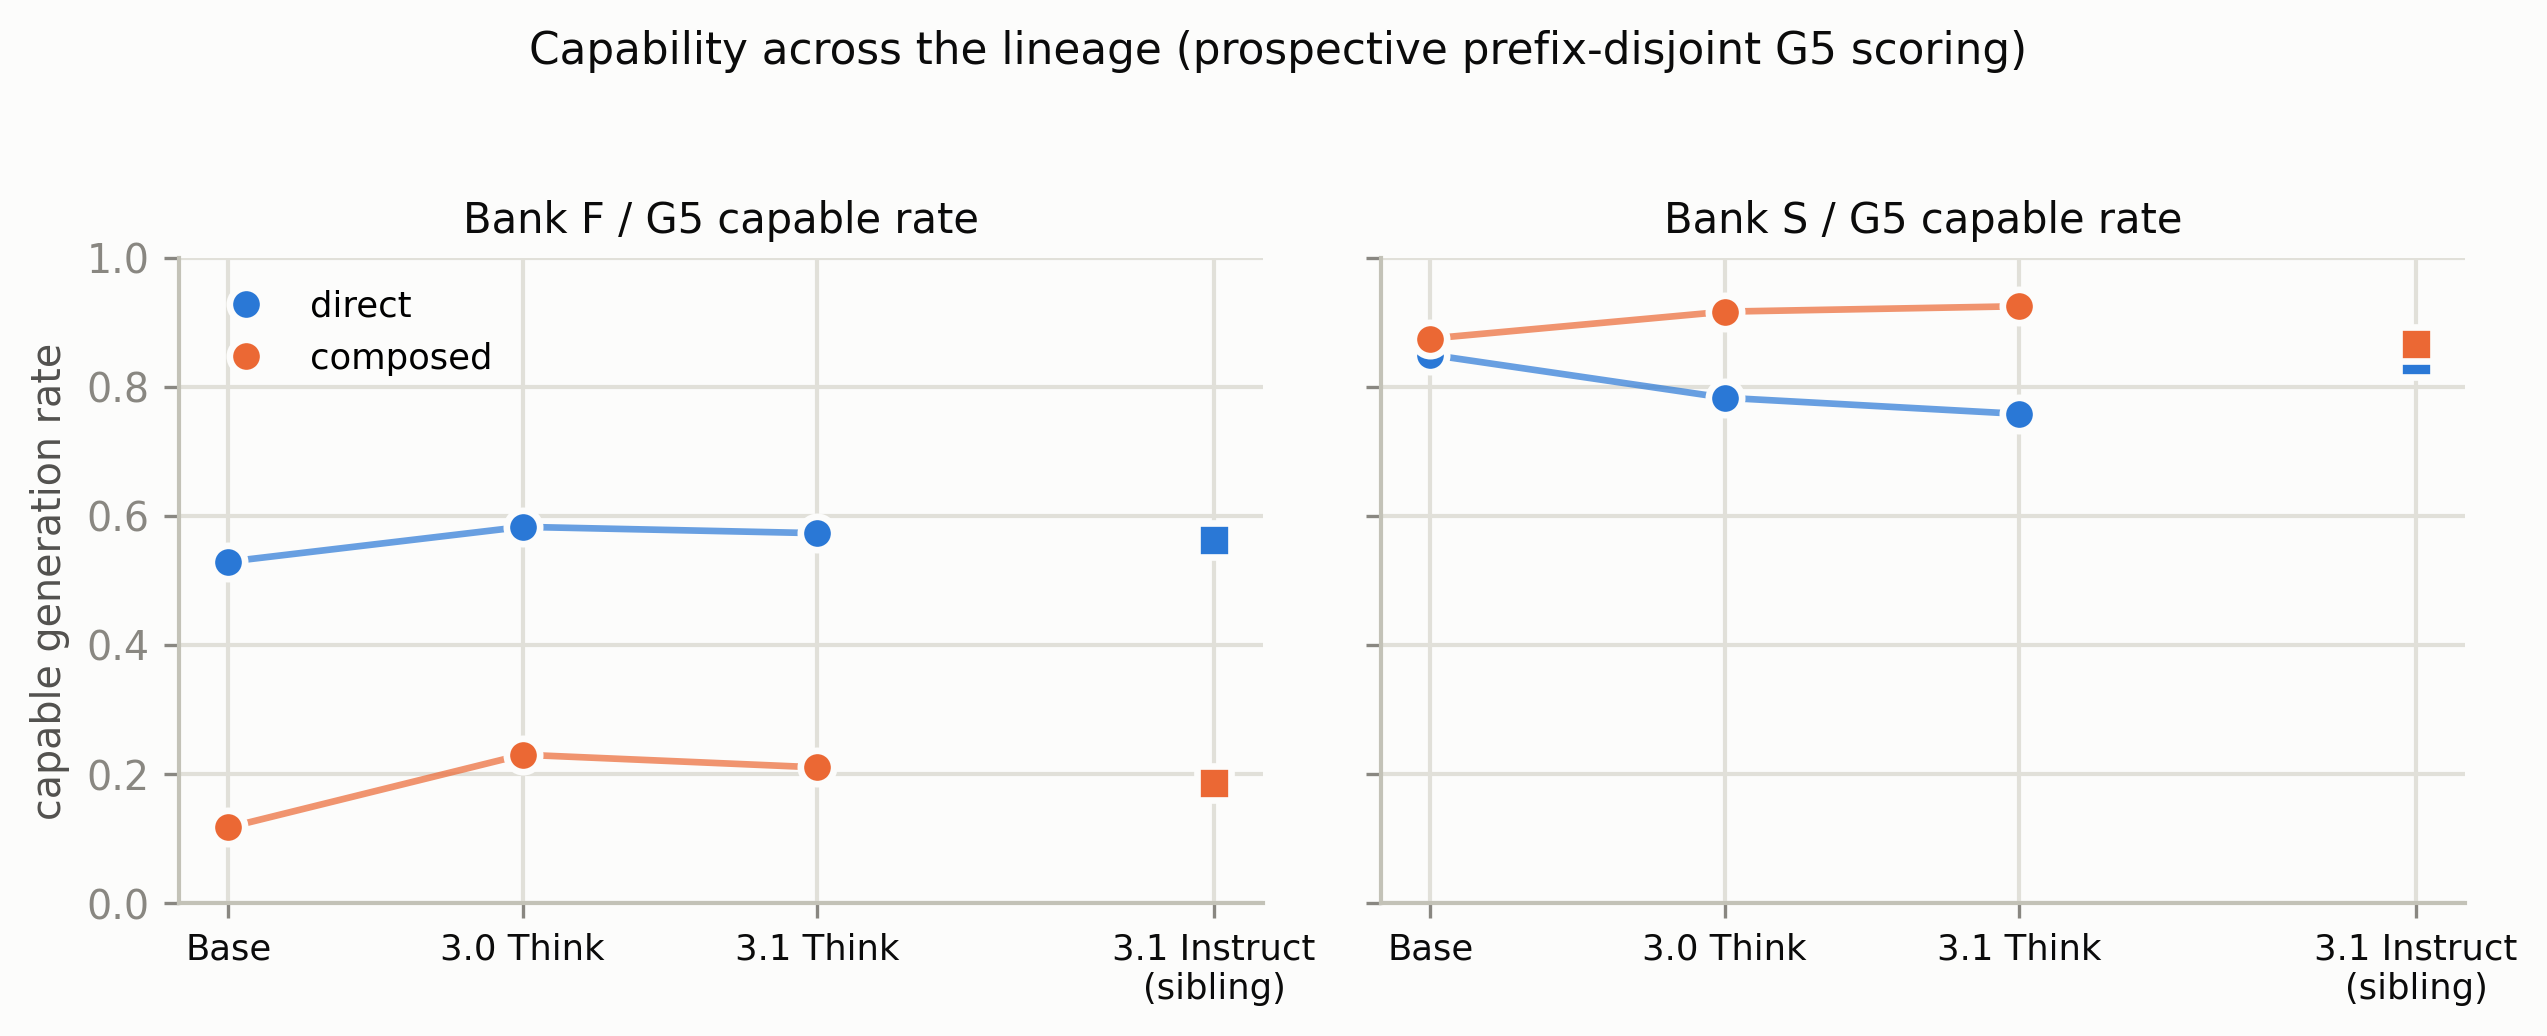
\includegraphics[width=0.94\textwidth]{olmoL2_capability_trajectory.png}
\caption{Prospective G5 capable-generation rates by checkpoint, bank, and
variant. Squares mark the Instruct sibling. The Think path does not simply
improve every task: Bank-S direct capability declines while Bank-S composed
capability rises. Evidence: \texttt{p4-g5-bank-*-dev-v*}.}
\label{fig:capability}
\end{figure}

Three observations matter for interpreting intervention effects:
\begin{itemize}
  \item Bank-F composition is hard at every checkpoint. The fact-bank
  development cohorts are direct-heavy, so Bank-F lineage claims remain
  imprecise and coordinate-sensitive.
  \item Bank-S direct capable rate falls from about 0.85 at base to 0.78 at
  3.0 Think and 0.76 at 3.1 Think, while composed rises from about 0.88 to
  0.92. The Instruct sibling sits nearer the base on both.
  \item Binary capability and conditional answer margin are not the same.
  On common-support facts, direct answer margin rises Base$\to$3.0 Think by
  $+1.95$ nats and again by about $+0.55$ to 3.1 Think even though the binary
  direct-capable rate falls \eid{p4-lineage-common-cohort-analysis-olmo-dev-v1}.
\end{itemize}

Capability membership was fixed before intervention outcomes at each
checkpoint. The common-support closure in \cref{sec:common-support} then asks
whether the trajectory survives when the exact same facts are forced into the
comparison.

\subsection{Base: no span-safe content-specific dependence}

At base, all four primary $\SJ$ cells are near zero:
Bank-F direct $+0.0245$ \ci{-0.0330}{+0.0792}, Bank-F composed $+0.0145$
\ci{-0.1226}{+0.1881}, Bank-S direct $+0.0005$
\ci{-0.0487}{+0.0481}, and Bank-S composed $+0.0021$
\ci{-0.0309}{+0.0385} \eid{p4-lineage-analysis-olmo3-base-dev-v1}.
The Bank-S composed-minus-direct contrast is $+0.0016$
\ci{-0.0417}{+0.0403}.

This is not a dead assay. The same base grid produces a positive overall
label-protected J-specific effect ($+0.123$) and nonzero mechanics-random and
logit-protected effects with intervals excluding zero. The instrument can move
the model; what is absent is dependence on the \emph{span-safe lens-selected
content} in these four cells.

\subsection{Think path: direct dependence appears by 3.0 and persists at 3.1}

By 3.0 Think, Bank-S direct $\SJ$ is $-0.128$
\ci{-0.207}{-0.049} in the own frame and $-0.097$
\ci{-0.156}{-0.045} in the frozen base frame. Bank-S composed is also
negative in both frames. At 3.1 Think, direct dependence remains negative
($-0.167$ own; $-0.155$ common) while the composed-minus-direct contrast
becomes precise and positive: $+0.118$ \ci{+0.052}{+0.188} own and $+0.117$
\ci{+0.028}{+0.209} common
\eid{p4-lineage-analysis-olmo31-think-dev-v2,p4-lineage-trajectory-analysis-olmo-dev-v1}.

The observed transition is not gradual in the available checkpoints. On
paired common-support facts there is no resolved 3.0$\to$3.1 Think increment.
The main localization is the wide base$\to$Think interval.

\subsection{Instruct sibling: the Bank-S pattern returns toward zero}

At OLMo-3.1 Instruct, Bank-S direct is $-0.022$
\ci{-0.066}{+0.018}, composed is $-0.018$
\ci{-0.076}{+0.033}, and their contrast is $+0.005$
\ci{-0.041}{+0.050} \eid{p4-lineage-analysis-olmo31-instruct-dev-v1}.
Every Bank-S interval includes zero in both the own and frozen-base frame.
This is a sibling reversal, not evidence that Instruct has no internal content:
Phase 3's frozen fact-item span audit found a substantial Instruct content
residual on a different population. The defensible statement is task- and
population-specific.

\begin{figure}[H]
\centering
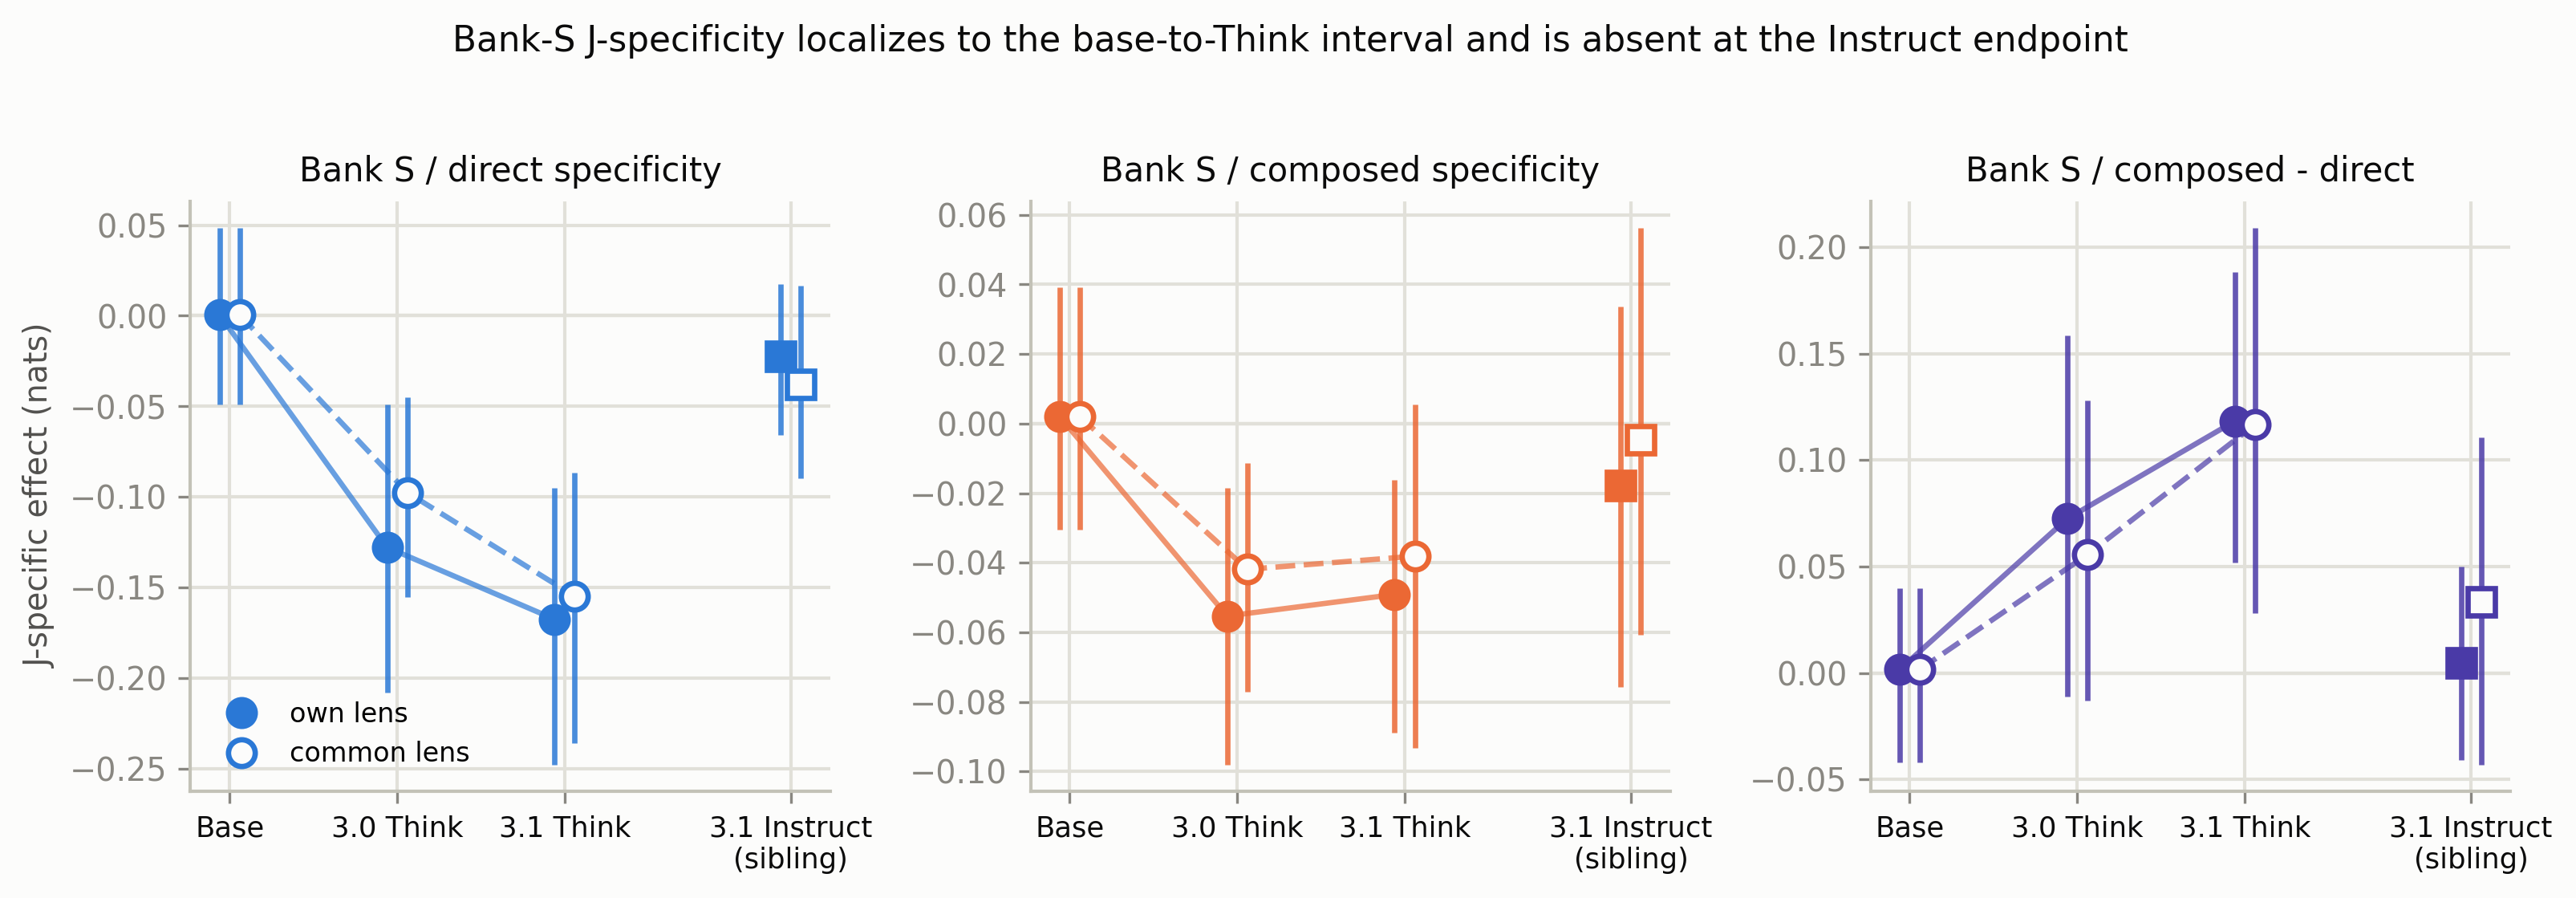
\includegraphics[width=0.97\textwidth]{olmoL1_emergence_trajectory.png}
\caption{Bank-S J-specificity along the observed OLMo graph. Filled markers
use each checkpoint's own lens; open markers use the frozen base lens. Lines
connect only Base $\to$ 3.0 Think $\to$ 3.1 Think; the Instruct square is a
sibling endpoint. Evidence: \texttt{p4-lineage-trajectory-analysis-olmo-dev-v1}.}
\label{fig:emergence}
\end{figure}

\subsection{A state-space view makes the training pattern clearer}

\begin{figure}[H]
\centering
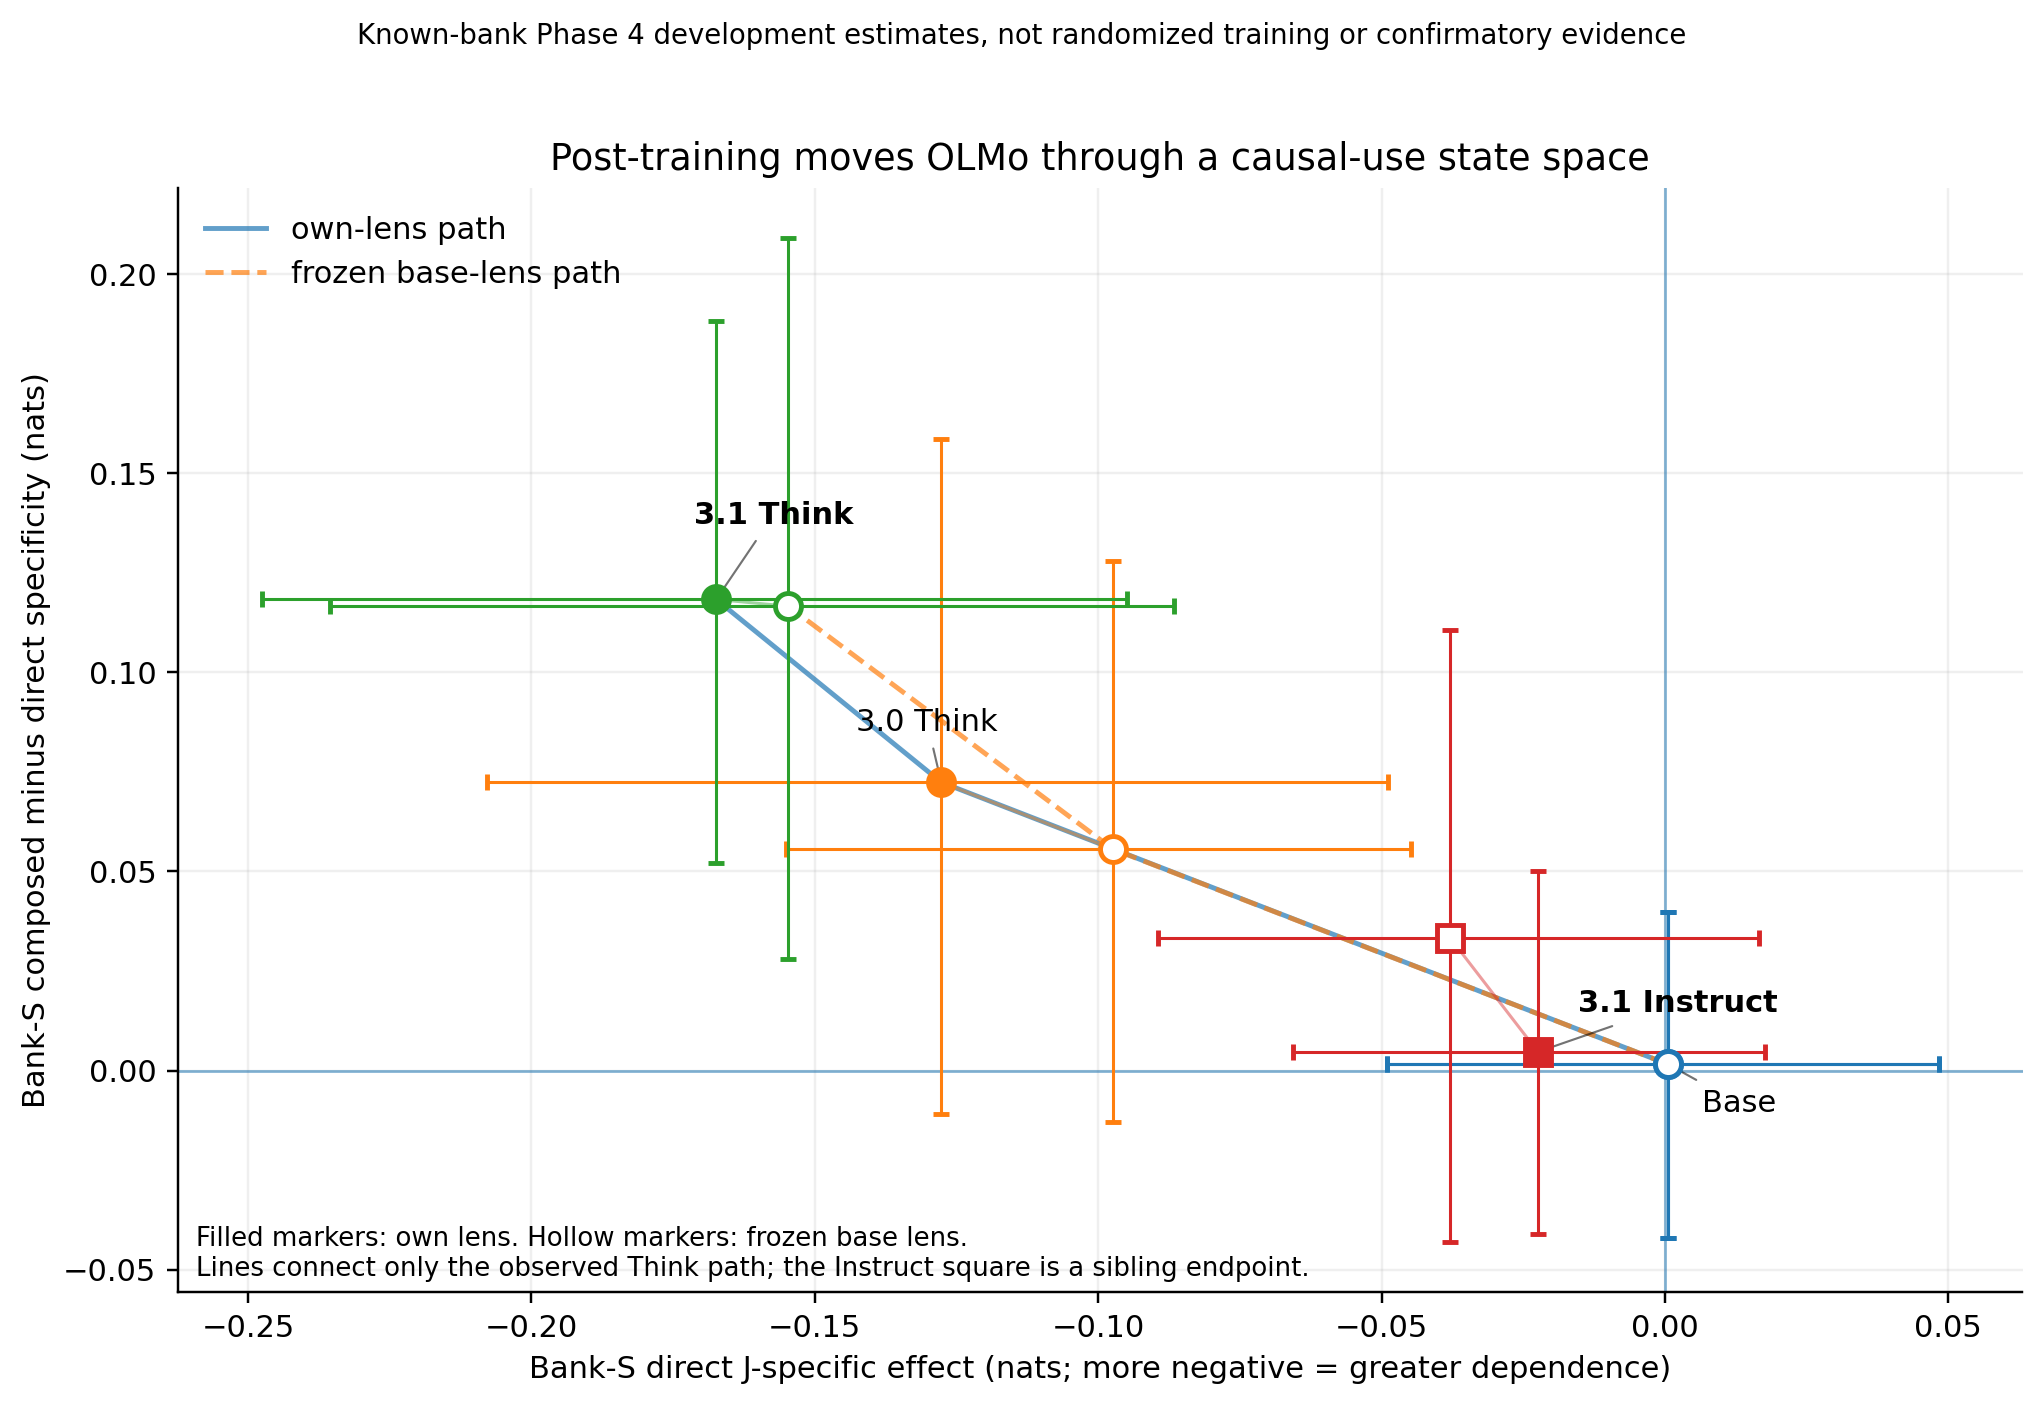
\includegraphics[width=0.94\textwidth]{olmoL5_training_state_space.png}
\caption{The lineage in a causal-use state space. Moving left means greater
Bank-S direct dependence; moving up means composed prompts are relatively less
dependent than direct prompts. The Think path leaves the base near the origin,
then moves left and upward; the Instruct sibling returns near the origin. Small
within-checkpoint connectors show own/common coordinate displacement. The
figure is regenerated from the registered trajectory CSV by the supplied
\texttt{olmo\_lineage\_synthesis\_plots.py}.}
\label{fig:state-space}
\end{figure}

\begin{resultbox}
The simplest description of the observed trajectory is not ``the workspace
gets bigger.'' It is: \textbf{the Think branch recruits a thin J-readable
channel for Bank-S direct state, while composed in-context state becomes
relatively less dependent on that channel; the Instruct sibling does not show
the same organization.} This is a statement about causal use under a specific
assay and task population, not a statement that a consciousness-style
workspace was created.
\end{resultbox}

%======================================================================
\section{What post-training changes, and what stays nearly fixed}\label{sec:change}

\subsection{The moving arm is J-selected content, not matched dose}

Because $\SJ=\dJ-\dC$, a trajectory could be manufactured by a wandering
control. The raw arms rule that out.

\begin{figure}[H]
\centering
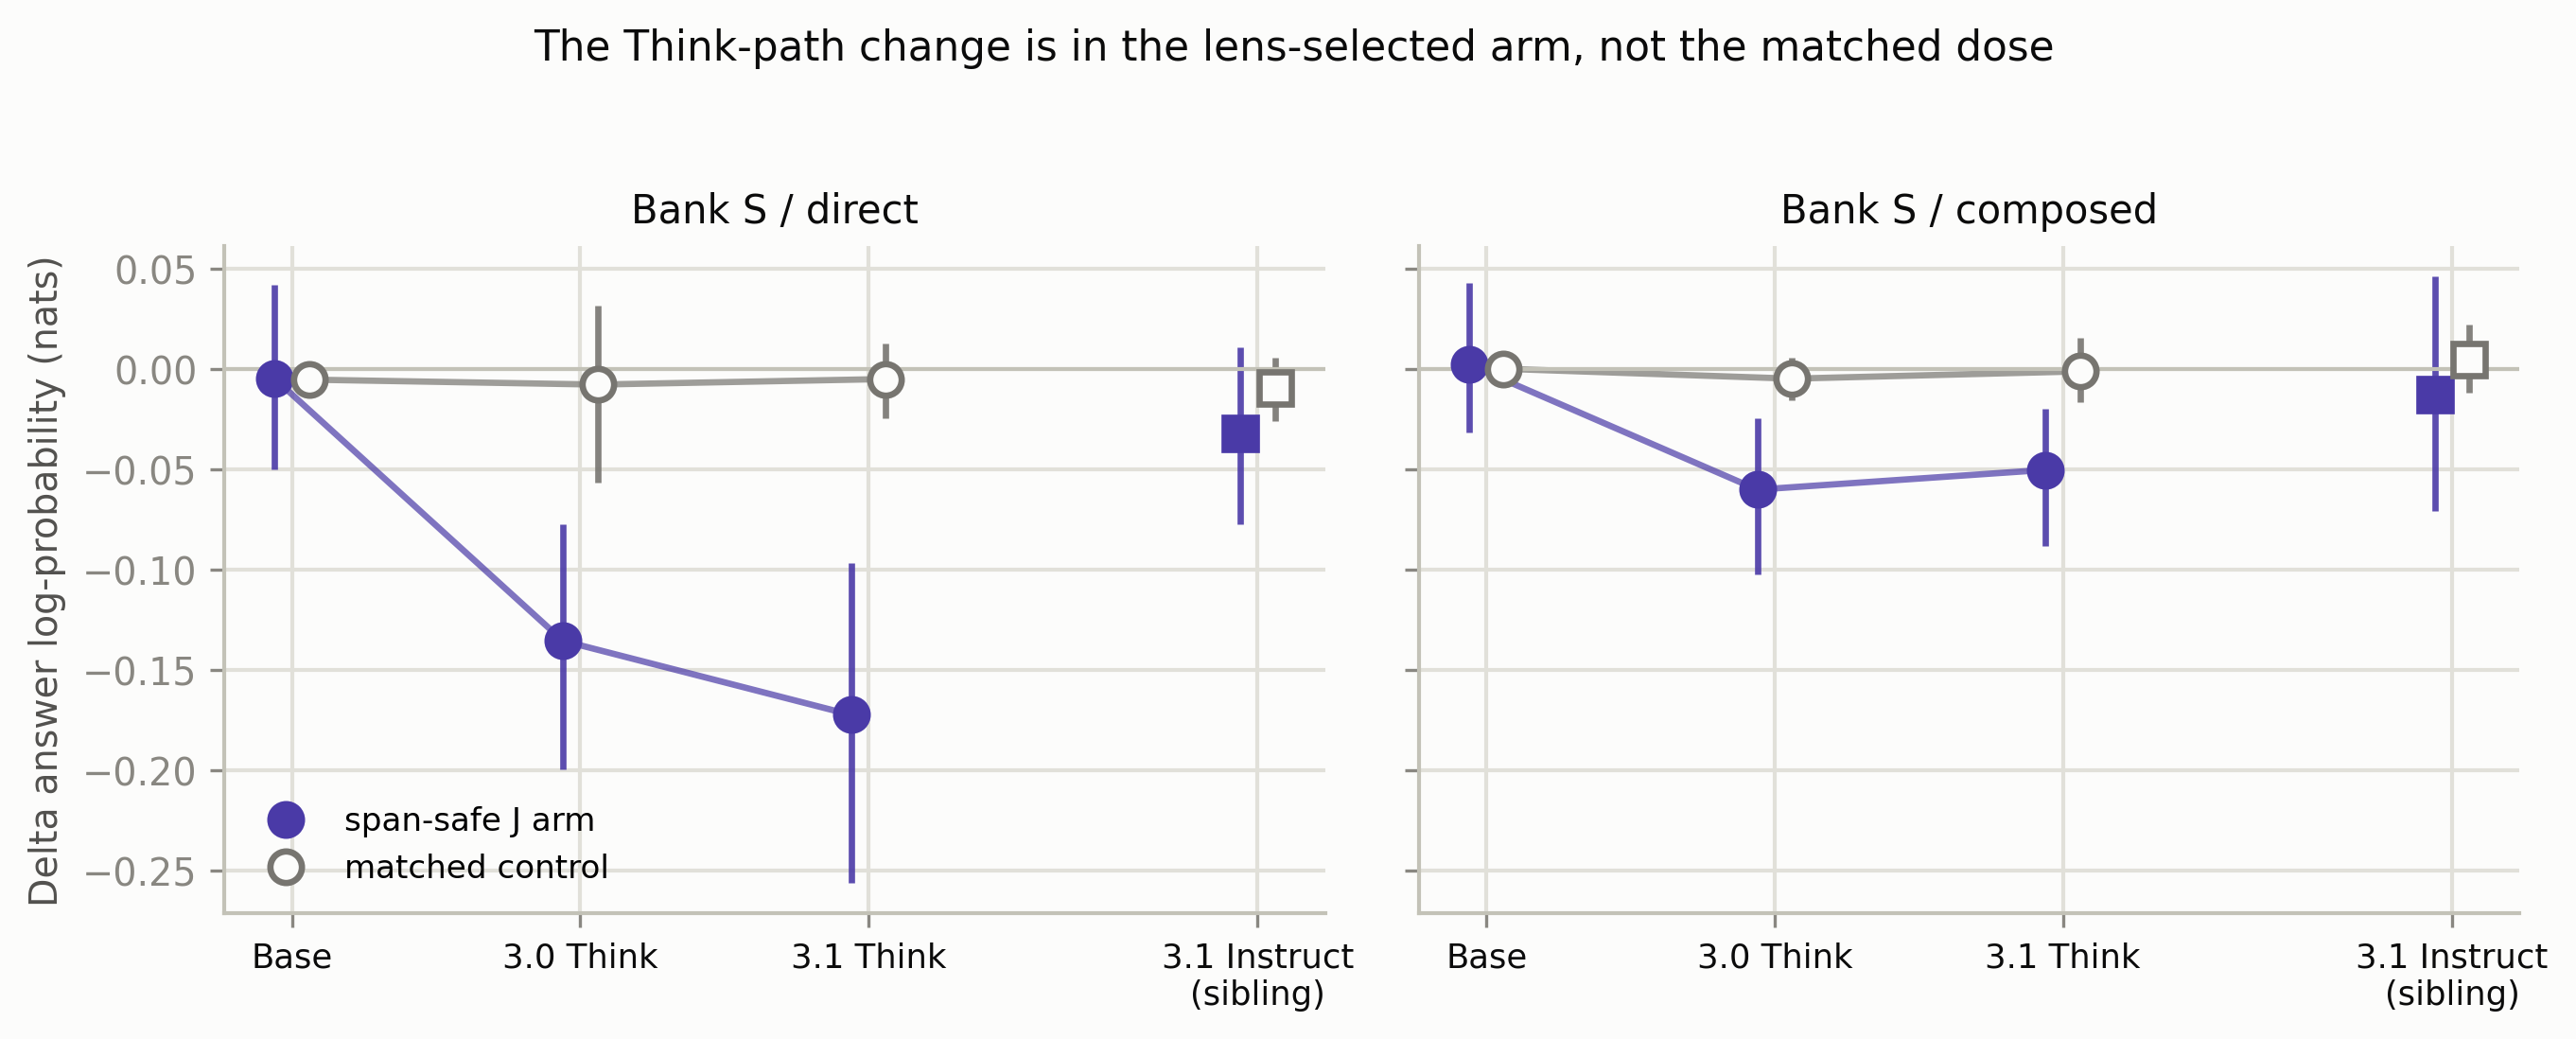
\includegraphics[width=0.98\textwidth]{olmoL3_bank_s_arm_decomposition.png}
\caption{Raw Bank-S intervention effects before subtraction. The span-safe J
arm moves from near zero at base to negative values at both Think checkpoints,
then rebounds at Instruct. The exact matched control remains near zero in every
cell. The training-path signal is carried by the selected content, not by a
generic fragility to matched-rank, matched-energy lesions.}
\label{fig:arms}
\end{figure}

For direct Bank S, base$\to$3.0 Think moves the J arm by roughly $-0.13$ nats
while the control moves only a few thousandths. Think$\to$Instruct reverses
the J arm by about $+0.14$ with essentially no control movement. This rules
out ``Think is simply more lesion-sensitive'' as the main account.

\subsection{Measured capacity is almost unchanged across post-training}

\begin{figure}[H]
\centering
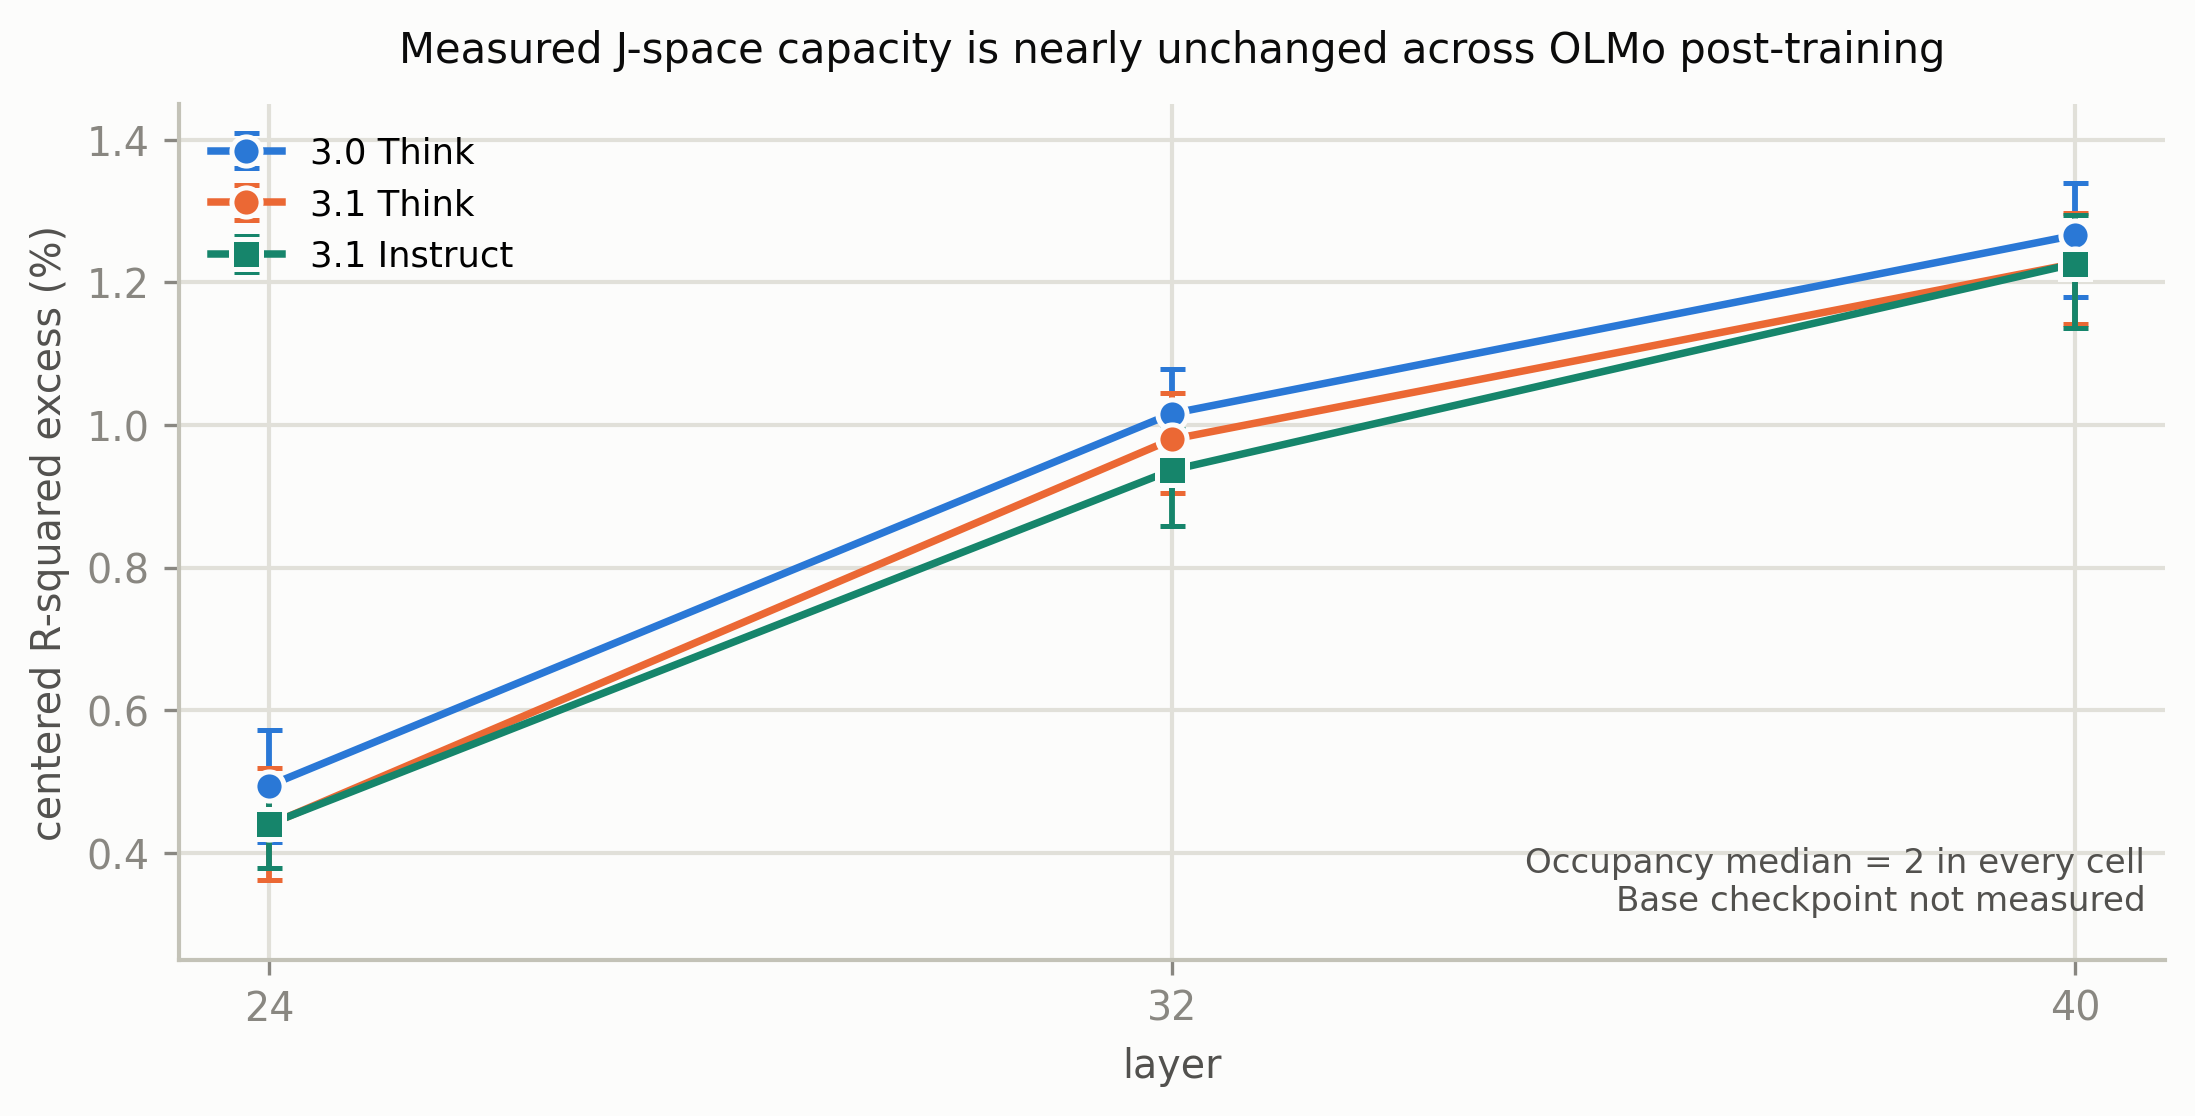
\includegraphics[width=0.91\textwidth]{olmoL4_capacity_posttraining.png}
\caption{Paper-defined capacity for the three measured post-training OLMo
checkpoints. Centered excess variance is approximately 0.44--0.49\% at L24,
0.94--1.02\% at L32, and 1.23--1.27\% at L40; occupancy median is 2 in every
cell. The base checkpoint has not yet been measured. Evidence:
\texttt{r2-occupancy-*-v2}.}
\label{fig:capacity}
\end{figure}

The 3.1 Think and Instruct capacity curves are nearly superposed even though
their common-support Bank-S direct specificity differs by about 0.11--0.14
nats, depending on frame. The 3.0 Think checkpoint has the same occupancy and
only slightly larger centered excess at these layers. Capacity and causal
utilization are therefore empirically dissociated within this lineage.

\begin{resultbox}[title={Update: the base cell is now measured --- and conserved}]
The parallel-phase O2 estimator closed this gap symmetrically: the same
ordered 120-prompt corpus and 7{,}481 content positions at layers 24/32/40,
run at Base, 3.0 Think, 3.1 Think, and the Instruct sibling, with three
matched random dictionaries and 2{,}000 paired domain-stratified prompt
bootstraps \eid{ol-capacity-joint-dev-v1}. The preregistered base$\to$3.0
Think own-frame centered-excess difference is $+0.0154$ percentage points,
paired 90\% interval \ci{-0.0121}{+0.0435} (in points), and the occupancy
difference is \emph{exactly zero}; 46 of 48 classified rows are stable under
the frozen $\pm0.25$-point margin (two Base-common L40 sensitivities sit
unresolved at the equivalence edge). The registered verdict is
\texttt{broadly\_conserved\_capacity\_recruitment\_consistent}. The licensed
wording is bounded --- ``measured sparse capacity, this estimator, these
margins'' --- never literal equality or global coordinate conservation.
\end{resultbox}

\subsection{The effect does not require checkpoint-specific coordinates}

The common-frame test applies the frozen base J-lens to every checkpoint while
keeping stochastic controls paired. Bank-S effects preserve their sign and
most of their interval structure. At 3.1 Think, the composed-minus-direct
contrast is $+0.118$ in the own frame and $+0.117$ in the common frame; their
paired difference is $-0.002$ \ci{-0.055}{+0.050}. At 3.0 Think, both direct
and composed effects remain negative in both frames. At Instruct, both remain
near zero.

\begin{figure}[H]
\centering
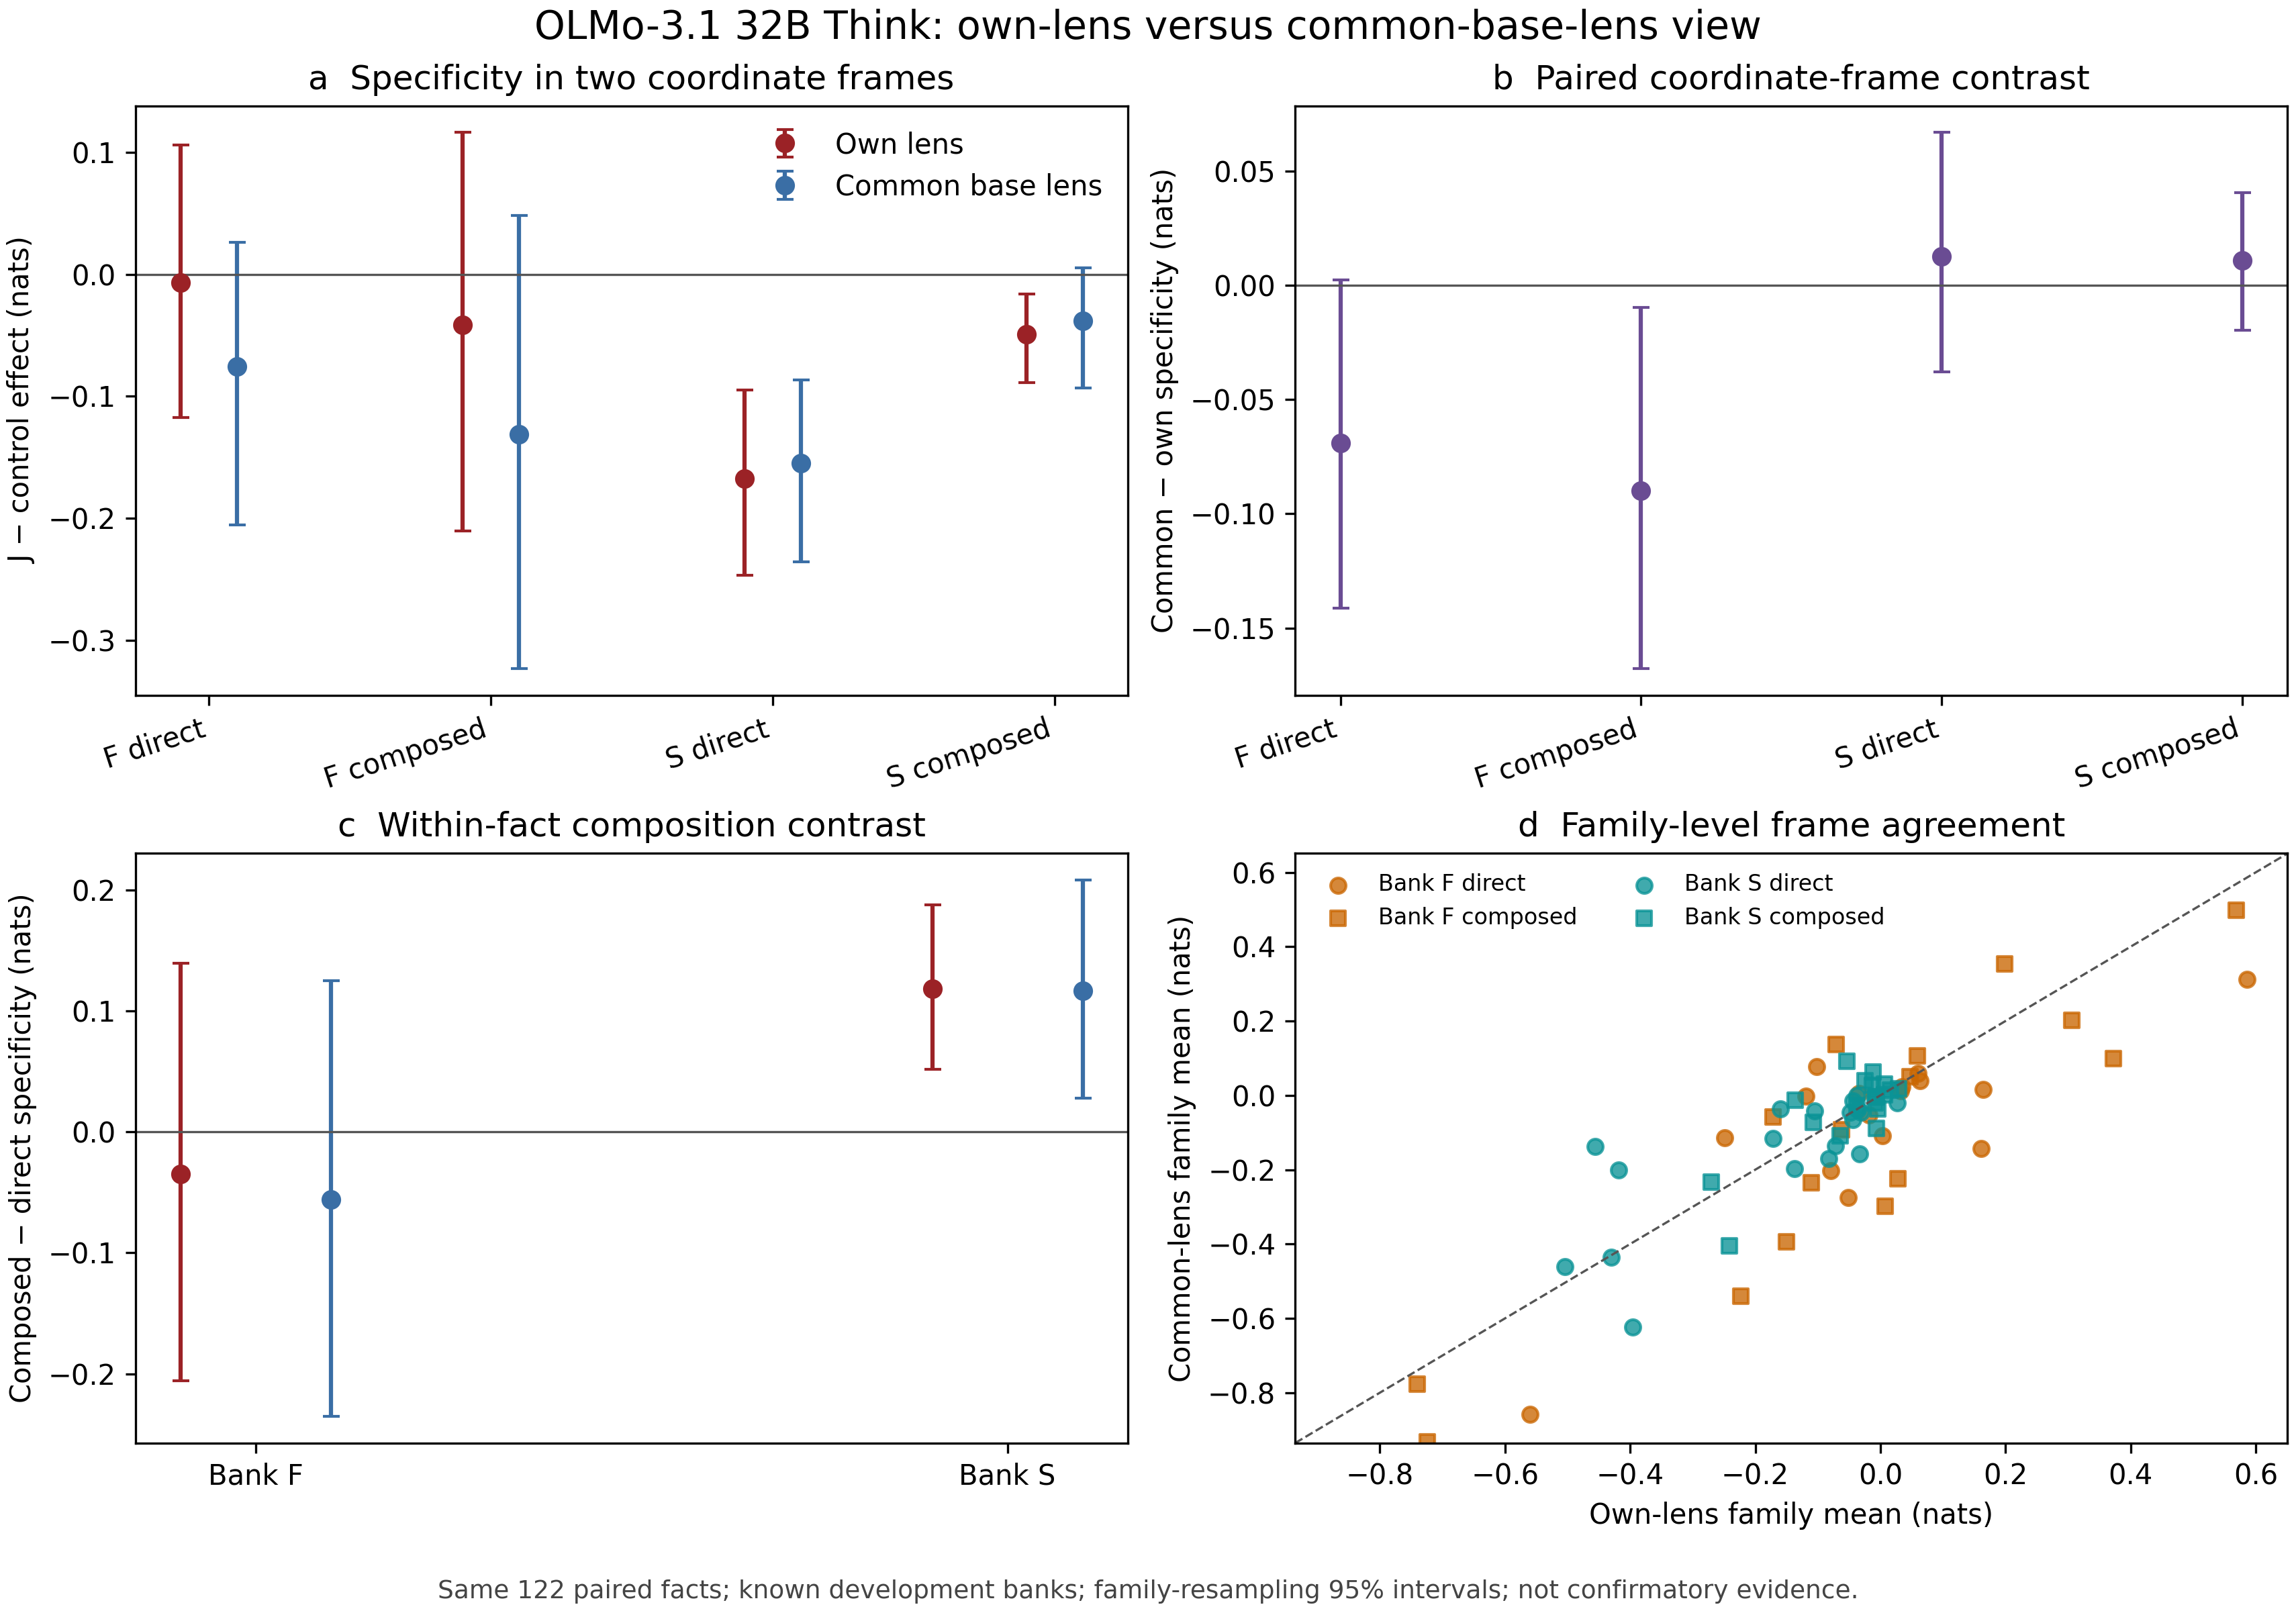
\includegraphics[width=0.91\textwidth]{p4f05_olmo31_think_lens_frame_comparison.png}
\caption{Seed-paired own-lens versus frozen-base-lens comparison at OLMo-3.1
Think \eid{p4-lens-frame-analysis-olmo31-think-dev-v1}. Bank-S aggregates are
stable across the two tested frames, while Bank-F contains the clearest
coordinate sensitivity.}
\label{fig:frame}
\end{figure}

This does not mean the dictionaries are identical. Item-level own/common
correlations are around 0.73--0.77 and mean absolute item shifts are
0.08--0.11 nats. The conclusion is narrower: checkpoint-specific lens
refitting is not necessary to recover the aggregate Bank-S training pattern.

\subsection{Readout coordinates transfer more readily than causal use}

Part 2 applied the 3.0 Think lens unchanged to OLMo-3.1 Instruct. The donor and
recipient retained the same 17/21 probe successes at rank $\le20$, nearly
identical pass@5/pass@20, median unembedding-row cosine 0.9984, and final-gain
cosine 1.000. The transfer lost some rank-1 sharpening, but preserved the
shortlist \eid{a0-transfer-gate-olmo31instruct-v1}.

\begin{figure}[H]
\centering
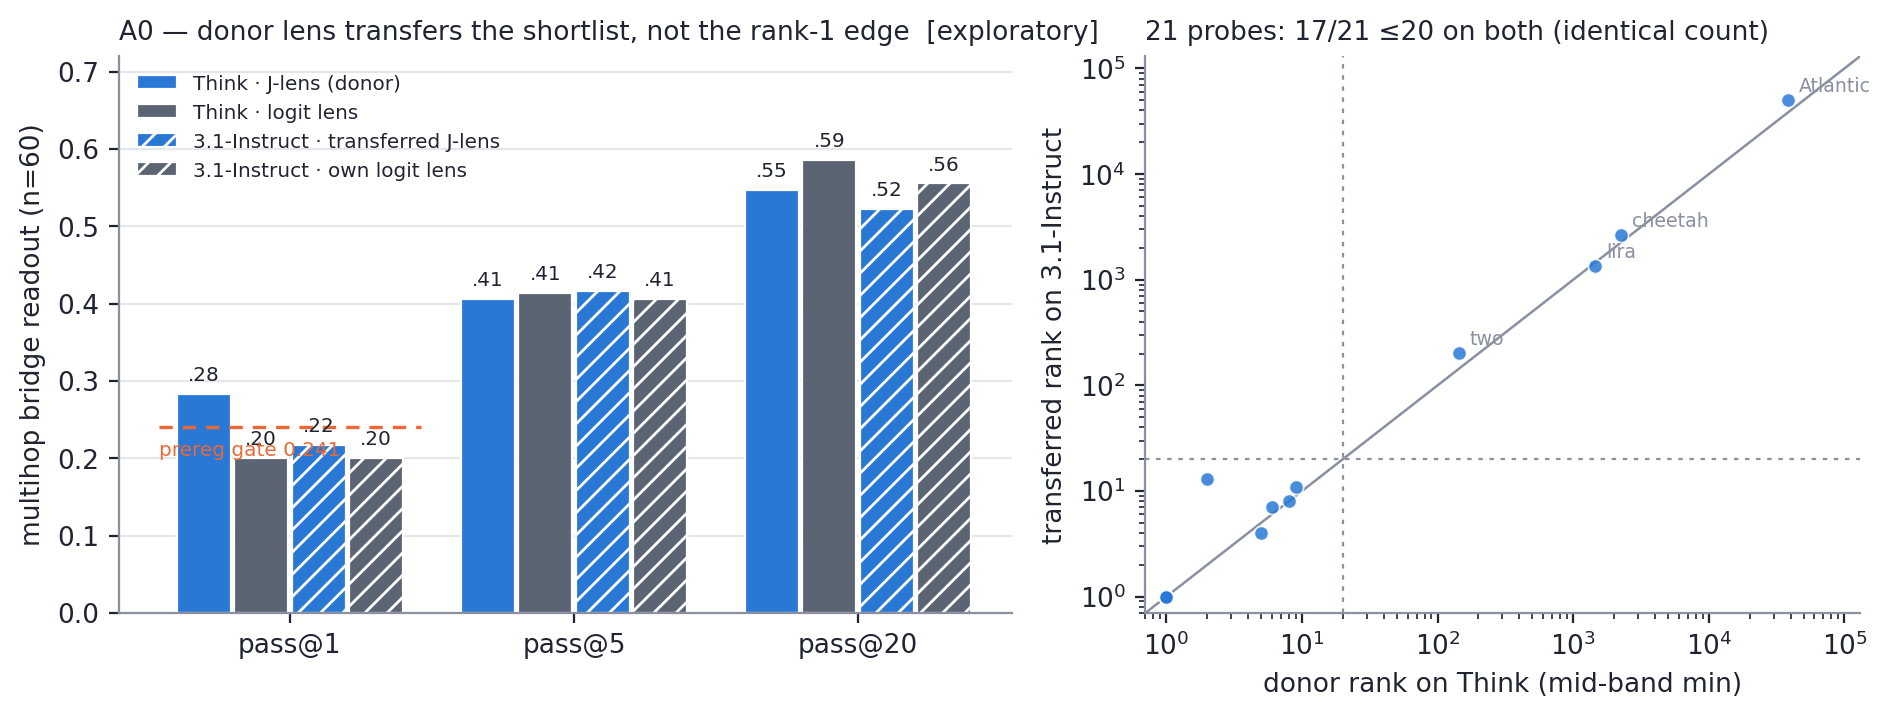
\includegraphics[width=0.98\textwidth]{p2f1_a0_transfer.png}
\caption{Exploratory donor-lens transfer. Post-training changes the sharp edge
of the readout more than the broad shortlist. This is geometry/readout evidence,
not a causal intervention comparison.}
\label{fig:transfer}
\end{figure}

The conjunction is informative: the broad verbalizable coordinate system
transfers, the measured capacity barely changes, and yet causal use on Bank S
separates sharply. That is the empirical shape expected under
\textbf{recruitment or rerouting of a conserved representation}.

\subsection{Direct same-corpus geometry: a dictionary-formation pattern}

The parallel phase replaced frame-transfer inference with direct geometry:
a lens-provenance audit first certified all six lens pairs as exact same
recipe and corpus (\texttt{EXACT\_SAME\_RECIPE\_CORPUS}, so no refit artifact
can explain a difference) \eid{ol-lens-provenance-audit-v1}, then the joint
geometry producer compared all 21 source layers across all six checkpoint
pairs, with exhaustive selected-span geometry at the 7{,}481 aligned
positions of layers 24/32/40 \eid{ol-geometry-joint-dev-v1}.

\begin{figure}[H]
\centering
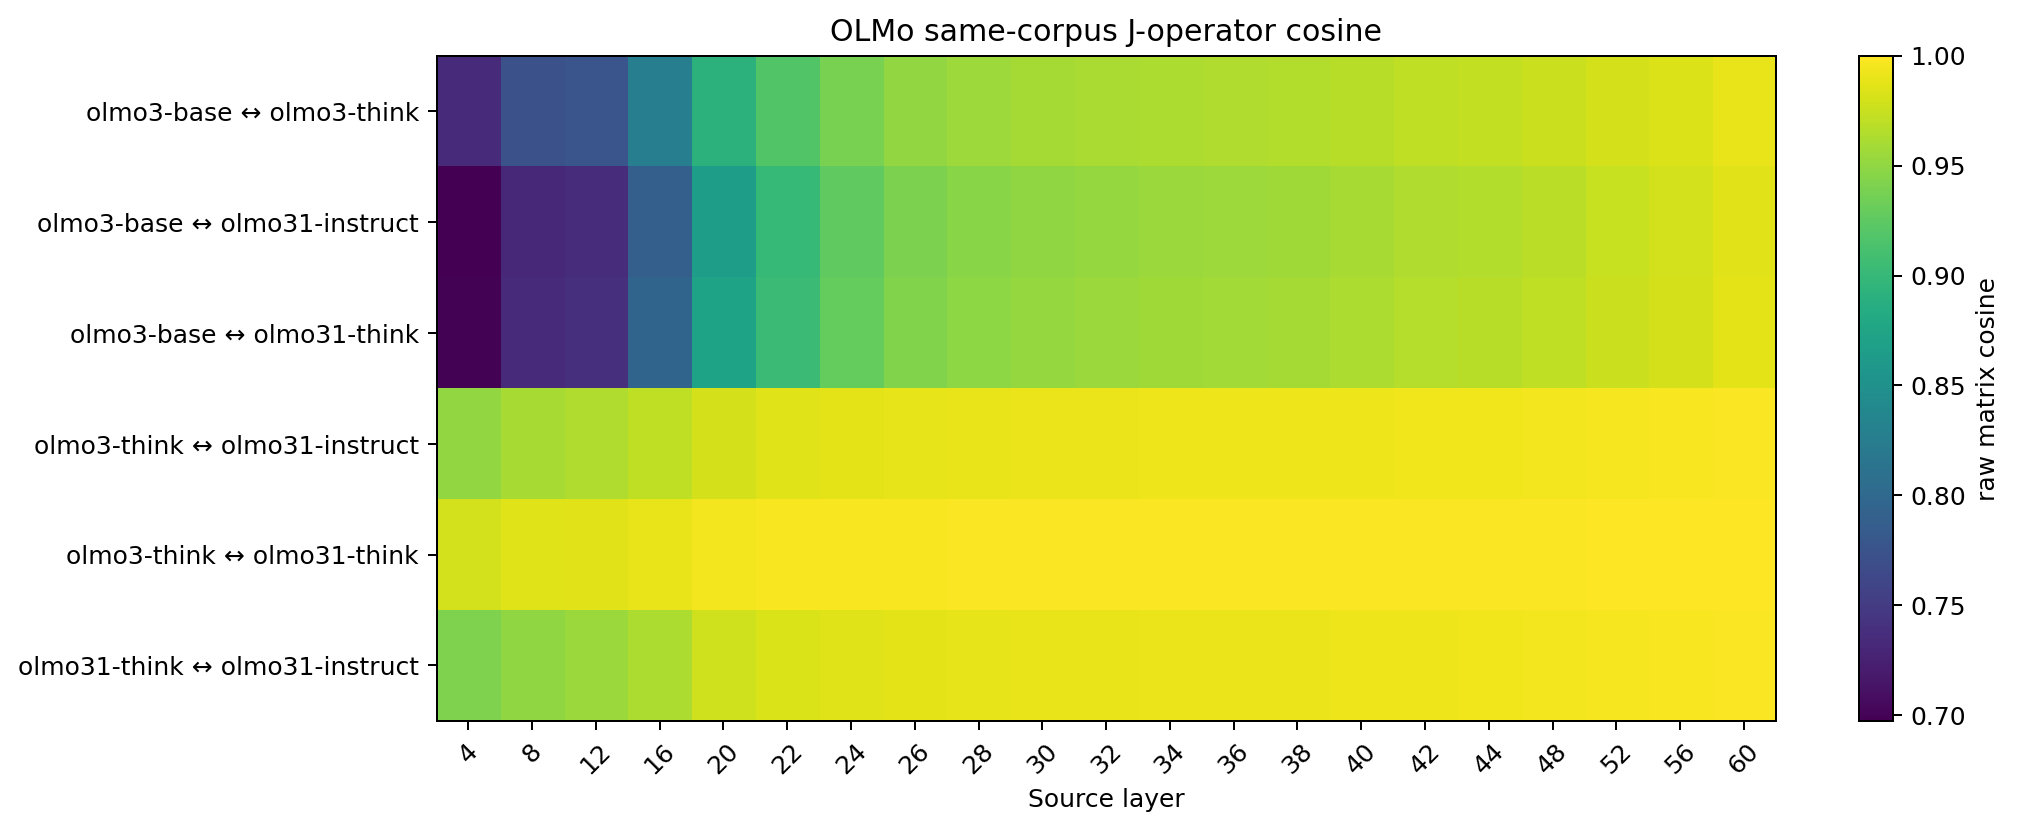
\includegraphics[width=0.93\textwidth]{olf01_operator_similarity_heatmap.png}
\caption{Registered O3 figure 1: raw-operator similarity across checkpoint
pairs and layers \eid{ol-geometry-figures-dev-v1}. The transport operators
stay broadly similar everywhere (base$\to$3.0 median cosine 0.9614).}
\label{fig:olf01}
\end{figure}

\begin{figure}[H]
\centering
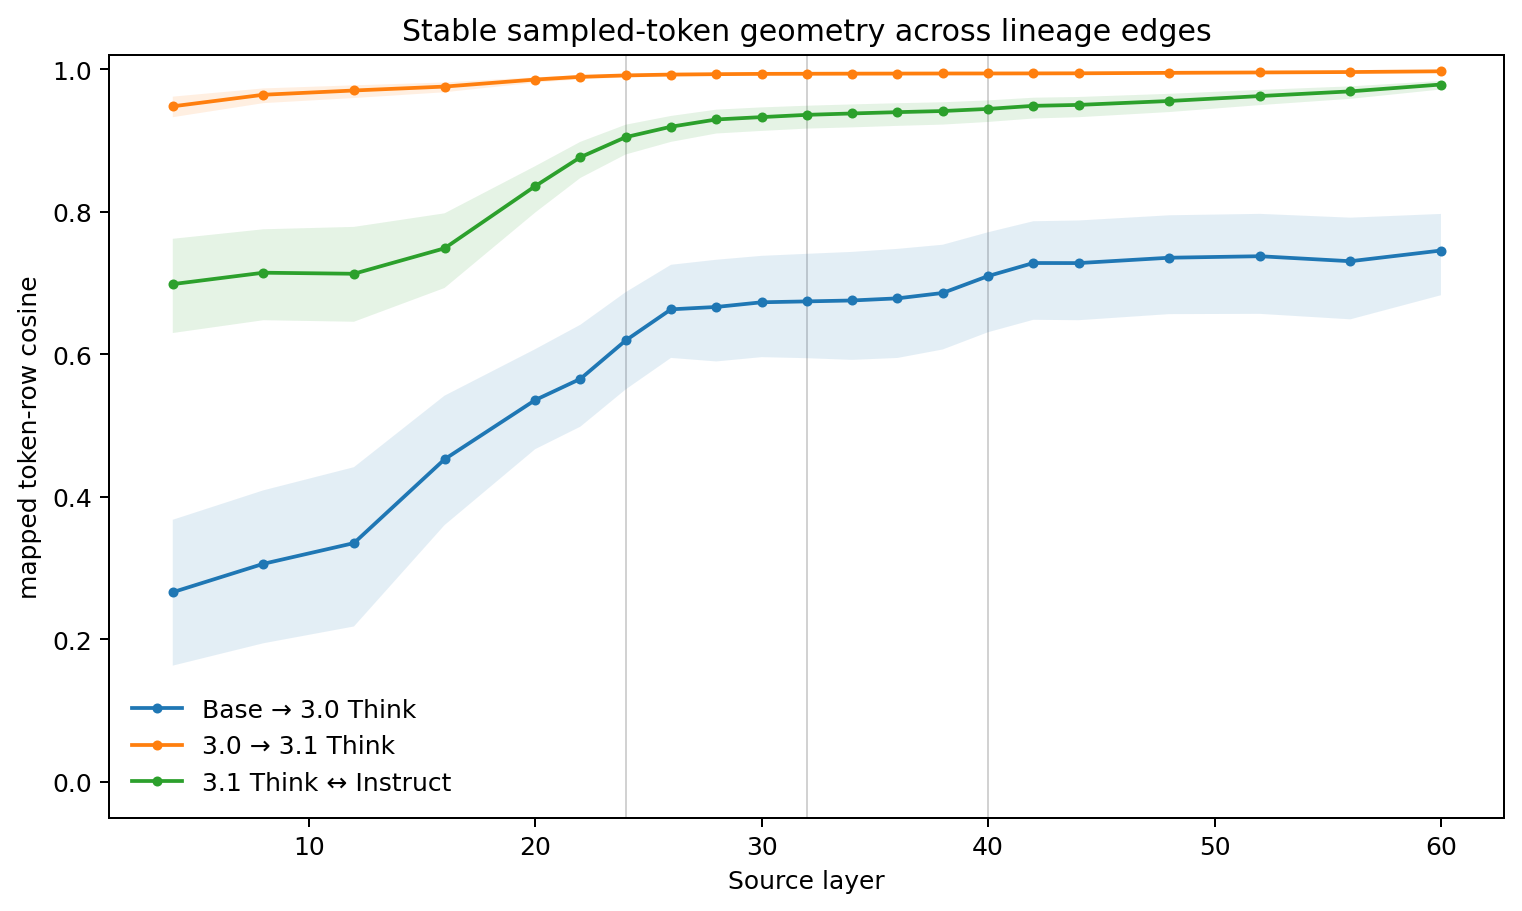
\includegraphics[width=0.93\textwidth]{olf02_token_row_similarity.png}
\caption{Registered O3 figure 2: J-\emph{mapped token-row} similarity. Unlike
the raw operators, the mapped rows reorganize sharply at base$\to$3.0
(median cosine 0.6744) and then freeze (3.0$\to$3.1 mapped movement 0.006
versus 0.326 for base$\to$3.0) \eid{ol-geometry-figures-dev-v1}.}
\label{fig:olf02}
\end{figure}

\begin{figure}[H]
\centering
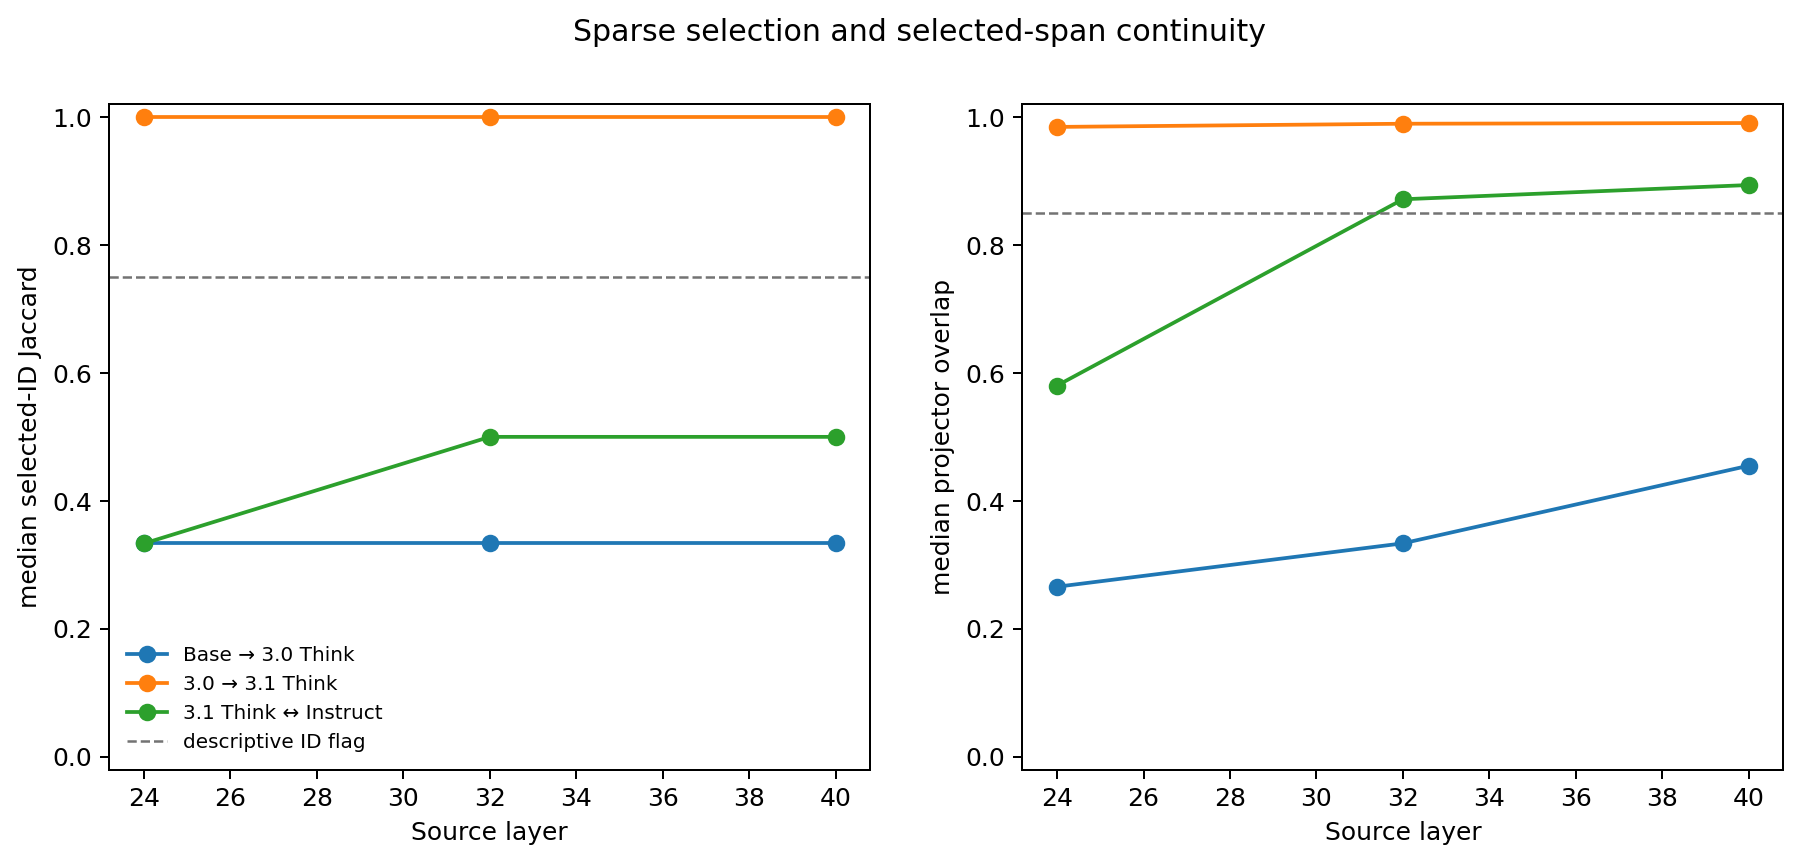
\includegraphics[width=0.93\textwidth]{olf03_selected_span_trajectory.png}
\caption{Registered O3 figure 3: what the assay actually selects. Base$\to$3.0
selected-ID Jaccard is 0.3333 at layers 24/32/40 (projector overlap
0.27/0.33/0.45); 3.0$\to$3.1 Jaccard is 1.0 at the same layers
\eid{ol-geometry-figures-dev-v1}.}
\label{fig:olf03}
\end{figure}

The frozen router classifies this as a \textbf{dictionary-formation pattern}:
the operator persists, but which token directions it maps --- and which the
assay therefore selects --- is rewritten in the base$\to$3.0 interval and
essentially frozen afterwards. Two sibling facts complete the picture: the
3.1 Think/Instruct mapped-row median is 0.9363 with
\texttt{instruct\_late\_shift=false} \eid{ol-geometry-joint-dev-v1}, so the
siblings share nearly the same dictionary while differing in causal use; and
the reorganization is concentrated exactly where \cref{fig:emergence}
puts the causal emergence. Geometry moves where utilization moves --- an
association across released checkpoints, not a stage attribution.

%======================================================================
\section{Common-support closure: the same facts tell the same story}\label{sec:common-support}

Checkpoint-specific capability cohorts could make a false trajectory if
different facts survive at each model. The common-support analysis freezes
membership from metadata only, before reading intervention outcomes. Seventy-nine
facts across 25 families survive all four checkpoints; adjacent pairs retain
92--119 facts across 29--34 families
\eid{p4-lineage-common-cohort-analysis-olmo-dev-v1}.

\begin{figure}[H]
\centering
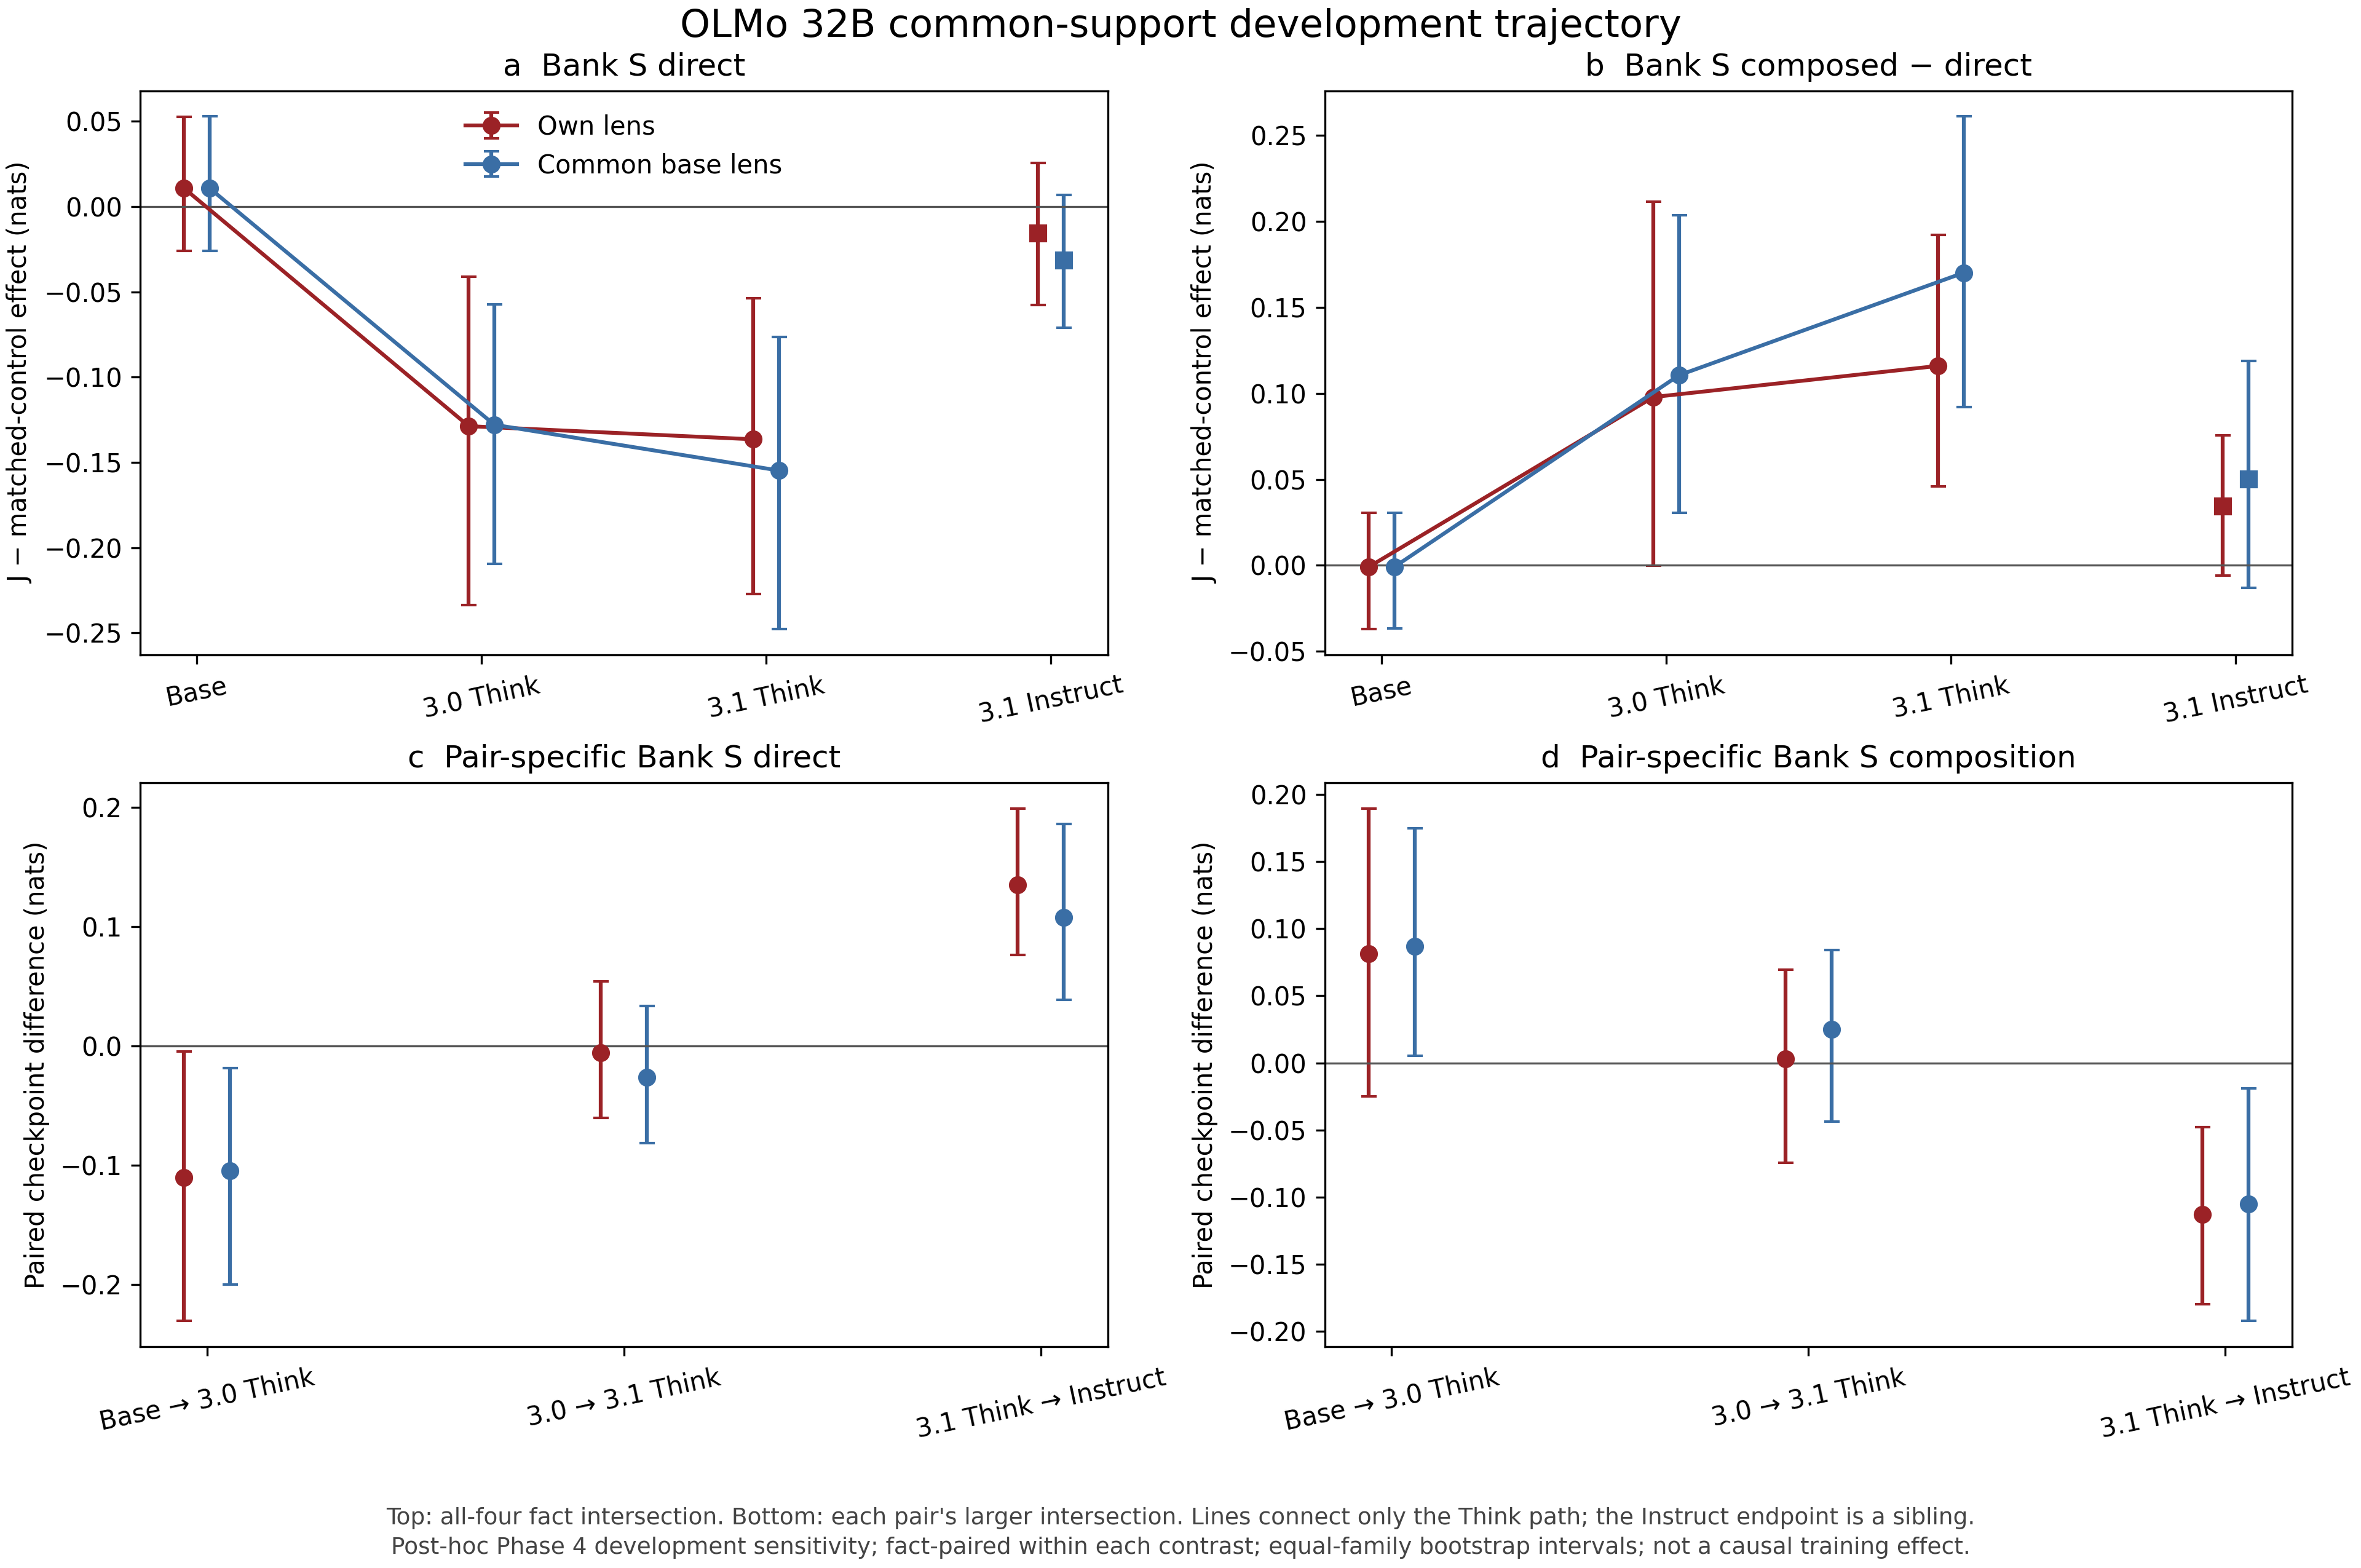
\includegraphics[width=0.99\textwidth]{p4f11_olmo_lineage_common_cohort.png}
\caption{Post-hoc common-support sensitivity. The upper panels use the
all-four intersection; the lower panels use larger adjacent-pair
intersections. This removes changing fact composition as one explanation,
but it does not randomize training.}
\label{fig:common-support}
\end{figure}

\begin{table}[H]
\centering\small
\begingroup
\setlength{\tabcolsep}{4.5pt}
\begin{tabular}{@{}lrrrr@{}}
\toprule
\textbf{Bank-S adjacent contrast} & \textbf{Own direct} & \textbf{Common direct} & \textbf{Own composition} & \textbf{Common composition}\\
\midrule
Base $\to$ 3.0 Think & $-0.110^{*}$ & $-0.105^{*}$ & $+0.081$ & $+0.087^{*}$\\
3.0 $\to$ 3.1 Think & $-0.006$ & $-0.027$ & $+0.003$ & $+0.025$\\
3.1 Think $\to$ Instruct & $+0.135^{*}$ & $+0.108^{*}$ & $-0.113^{*}$ & $-0.105^{*}$\\
\bottomrule
\end{tabular}
\endgroup
\caption{Right-minus-left checkpoint deltas on identical facts, equal-family
weighting, 100{,}000 family bootstraps. $^{*}$ marks a 95\% interval excluding
zero. ``Composition'' is the change in composed-minus-direct specificity.}
\label{tab:common-support}
\end{table}

The direct base$\to$Think decrease survives in both frames. The composition
increase has the same sign in both frames and excludes zero in the common
frame. No additional 3.0$\to$3.1 Think change is resolved. The sibling
Think$\to$Instruct comparison reverses both direct dependence and the
composition contrast in both frames, with all four intervals excluding zero.
Every one-family-out estimate preserves the signs of the emergence and the
reversal.

Baseline-answer-LP adjustment keeps the common-frame base$\to$Think direct
change below zero but widens several other intervals. Capability is therefore
tracked as a moderator rather than declared irrelevant. The closure shows
that changing fact membership is not sufficient to explain the trajectory;
it does not prove the training recipe caused it.

%======================================================================
\section{The isolated parallel-phase release (August 2026)}\label{sec:parallel}

While mainline Phase 4 remained blocked on the Qwen lens ladder, an isolated
OLMo side track (package \texttt{interpretability/jspace\_olmo\_lineage},
evidence prefix \texttt{ol-}, own branch and Drive root, forbidden from
writing any Phase 4/Gemma registry) ran the lineage-specific program to a
hash-pinned release boundary \eid{ol-phase4-final-import-bundle-v1}. Its five
objectives resolved as follows.

\subsection{O1: the Bank-W service gate ran --- and failed honestly}
The frozen baseline-capability protocol scored the derived/once Bank-W cell
(24 families $\times$ 8 seeds $\times$ two loads, 384 rows per model, all
eight answer candidates scored by summed conditional log probability):

\begin{table}[H]
\centering\small
\begin{tabular}{@{}lrrrrr@{}}
\toprule
\textbf{Model} & \textbf{Low acc.} & \textbf{High acc.} & \textbf{High$-$low} & \textbf{90\% CI} & \textbf{Capable families}\\
\midrule
OLMo-3.1 Think & 0.7135 & 0.7188 & $+0.0052$ & \ci{-0.031}{+0.042} & 17/24\\
OLMo-3.1 Instruct & 0.7396 & 0.7188 & $-0.0208$ & \ci{-0.057}{+0.021} & 17/24\\
Qwen 3.6 27B (imported) & 0.8333 & 0.8333 & $0$ & $\approx$\ci{-0.021}{+0.021} & 20/24\\
\bottomrule
\end{tabular}
\caption{Bank-W capability service results
\eid{ol-bank-w-capability-*-dev-v1}. Both OLMo endpoints pass individually,
but the exact three-model intersection is 16 families against the prospective
minimum of 20.}
\label{tab:bankw-gate}
\end{table}

Consequently \texttt{olmo\_phase4\_service\_ready=false}: the O4 mechanism
factorial --- the experiment this document's hypothesis boxes kept deferring
to --- \textbf{never opened}. The four frozen accounts (external-state
substitution, generic difficulty, capacity, output-adjacent routing) were
neither selected nor rejected. Bank W version 1 is closed; any successor is a
new prospective protocol, not a subset of the failed cohort.

\subsection{O2/O3: capacity conserved, dictionary reorganized}
Covered in \cref{sec:change}: the symmetric four-checkpoint capacity table
(occupancy difference exactly zero; verdict
\texttt{broadly\_conserved\_capacity\_recruitment\_consistent}) and the
same-corpus geometry audit (router \texttt{dictionary-formation-pattern}).
The registered state-space figure places every checkpoint on both axes at
once:

\begin{figure}[H]
\centering
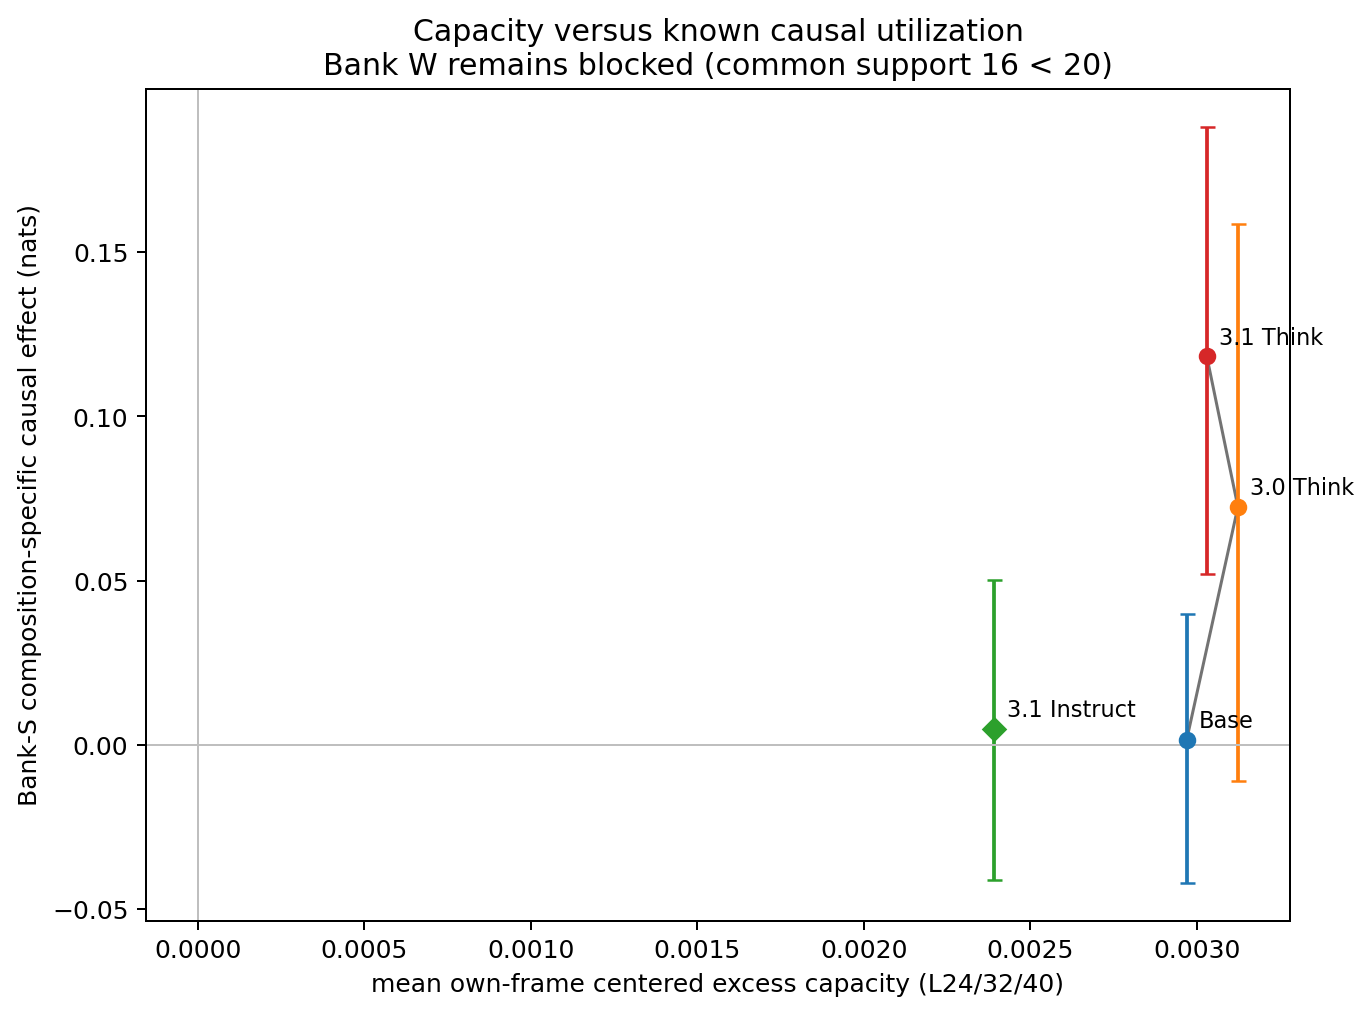
\includegraphics[width=0.9\textwidth]{olf04_capacity_causal_state_space.png}
\caption{Registered O3 figure 4: measured capacity versus known Bank-S causal
dependence, with the 16/20 Bank-W service block annotated
\eid{ol-geometry-figures-dev-v1}. The lineage moves almost entirely along the
causal axis.}
\label{fig:olf04}
\end{figure}

\begin{figure}[H]
\centering
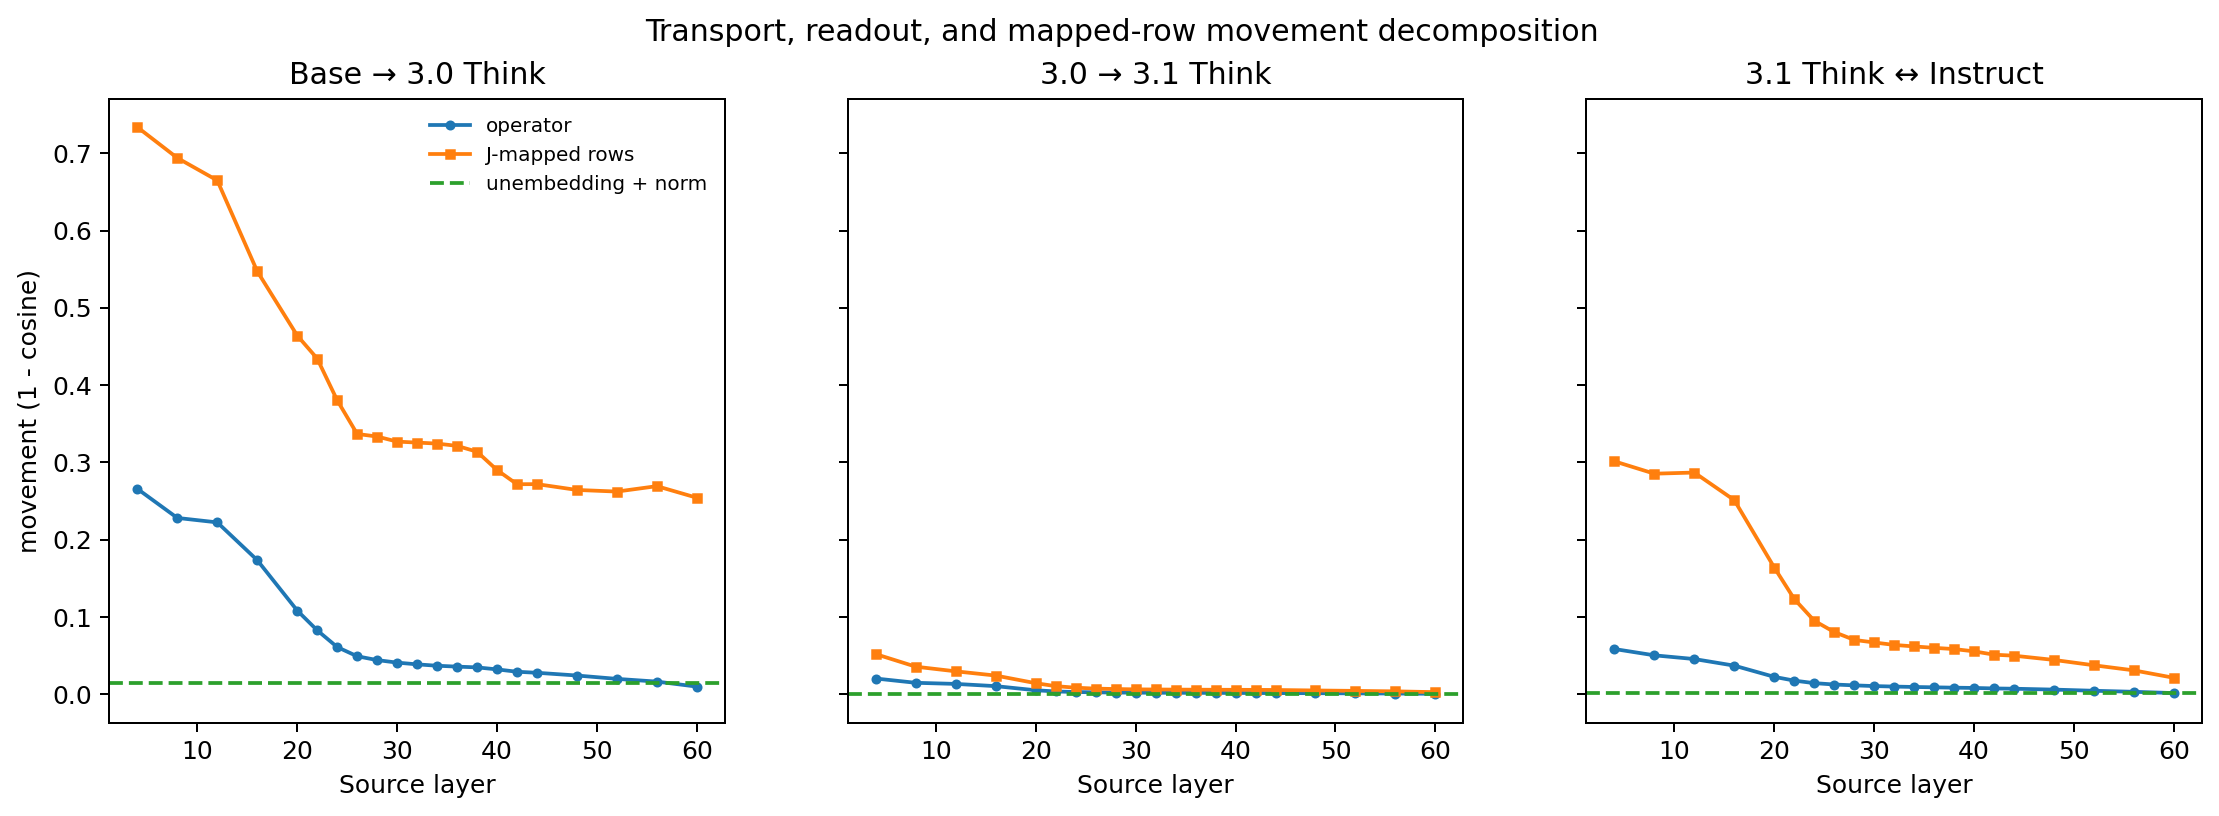
\includegraphics[width=0.9\textwidth]{olf05_readout_transport_decomposition.png}
\caption{Registered O3 figure 5: readout/transport movement decomposition
across the lineage \eid{ol-geometry-figures-dev-v1}.}
\label{fig:olf05}
\end{figure}

\subsection{Inventory, O5, and the reconstruction floor}
Three further dispositions matter for what comes next:

\begin{itemize}
  \item \textbf{Official intermediates exist} \eid{ol-checkpoint-inventory-v2}:
  a semantic tokenizer audit (superseding v1's byte-identity conservatism)
  finds the official 32B Think-SFT and Think-DPO artifacts eligible ---
  verdict \texttt{genuine-32b-intermediates-available}, H5
  \texttt{testable-with-bounded-stage-wedge}, queued. The ``wide interval''
  complaint in \cref{sec:next} now has a concrete two-cell wedge design.
  \item \textbf{O5 is not identifiable yet} \eid{ol-o5-feasibility-decision-v1}:
  the registry lacks crossed activation$\times$transport$\times$readout cells
  with the required transport, protected-span, rank/energy, and logit-lens
  controls, so the crossed causal decomposition returns
  \texttt{defer-no-identifiable-crossed-intervention-estimand} --- explicitly
  \emph{not} a null estimate. The bounded entry is a Bank-S-first
  Base/3.1-Think/3.1-Instruct pilot.
  \item \textbf{Everything reconstructs} \eid{ol-independent-reconstruction-v1}:
  768 O1 rows, all O2/O3 aggregates and bootstraps, five byte-identical PNGs,
  and one frozen model row replayed from the exact weight shards with maximum
  drift 0.
\end{itemize}

\begin{warningbox}
The release ledger narrows two paper-facing sentences, and these notes adopt
the narrowed forms verbatim. \textbf{Sentence 2} (training dependence):
``Across the tested, architecture-matched OLMo lineage, the first released
Think transition is associated with substantial reorganization of J-mapped
token and selected-span geometry without a material increase in measured
sparse capacity; the design does not identify which training ingredient
caused that change.'' \textbf{Sentence 4} (externalization): ``Existing
Bank-S development evidence motivates an external-state-substitution
hypothesis on the tested Think checkpoints, but the planned fact-paired
Bank-W factorial was gated out at 16/20 common families; this release does
not resolve an externalization mechanism.'' The original stronger candidates
must not be silently retained.
\end{warningbox}

%======================================================================
\section{What does ``J-space formation'' mean here?}\label{sec:formation}

A useful way to interpret the lineage is to separate three objects:
\[
\underbrace{D_{\theta,\ell}}_{\text{verbalizable coordinates}},\qquad
\underbrace{C_{\theta,\ell}}_{\text{capacity / occupancy}},\qquad
\underbrace{U_{\theta,\ell,T}}_{\text{causal utilization on task }T}.
\]
The fitted J dictionary $D$ describes a coordinate frame. Capacity $C$ asks
how much activation variance can be represented sparsely beyond matched random
controls. Utilization $U$ asks whether the selected content is causally needed
for a task after dose is matched.

\begin{table}[H]
\centering\small
\begin{tabularx}{\textwidth}{@{}p{0.22\textwidth}p{0.23\textwidth}X p{0.24\textwidth}@{}}
\toprule
\textbf{Formation hypothesis} & \textbf{Expected signature} & \textbf{Observed OLMo evidence} & \textbf{Current verdict}\\
\midrule
Larger workspace forms & occupancy or centered excess rises on Think & Occupancy difference exactly 0 including base; centered excess moves $+0.015$pp \ci{-0.012}{+0.043} \eid{ol-capacity-joint-dev-v1} & not supported on any measured checkpoint pair\\
New coordinate system forms & effect appears only under own Think lens; donor/common frame fails & The mapped token dictionary \emph{does} reorganize at base$\to$3.0 (row cosine 0.67, Jaccard 0.33) then freezes \eid{ol-geometry-joint-dev-v1} --- yet the aggregate effect survives the frozen base lens & real as reorganization; not necessary for detecting the effect\\
Existing channel is recruited & capacity and broad coordinates stable while $\SJ$ changes & J arm moves, matched control stays near zero; common-support, common-frame, conserved capacity, and dictionary-formation geometry all cohere & best-supported development account\\
Behavioral strategy changes only & capability/output formatting changes but causal channel does not & capability changes, but exact matched intervention dependence also changes & insufficient as a complete account\\
\bottomrule
\end{tabularx}
\caption{Different meanings of ``workspace formation.'' The current evidence
is most consistent with causal recruitment or rerouting of a channel whose
measured size is conserved but whose token dictionary reorganizes; the queued
official SFT/DPO wedge (H5) is what could turn the wide base$\to$3.0 interval
into a stage attribution.}
\label{tab:formation}
\end{table}

This distinction matters for the main paper. A model can retain a small,
readable coordinate system through post-training while changing which
computations write into it, how long content persists, which downstream
components read it, and whether prompt-supplied state substitutes for it.
Those are organization changes even if concept count and explained variance
stay flat.

%======================================================================
\section{Relation to the main paper, Qwen, and Gemma}\label{sec:comparison}

\subsection{The main paper's claim is a bundle, not one number}

The original workspace interpretation combines several properties: limited
capacity, verbalizable coordinates, broad downstream availability, causal
importance for multi-step behavior, and relative sparing of ordinary language.
This campaign supports some parts of that bundle more strongly than others.
It has strong evidence for verbalizable causal channels and exact-control
specificity. It does not currently support a selective global-workspace claim
for OLMo: prose damage is not cleanly spared, and the lineage result is
Bank-S/task-population specific.

\begin{figure}[H]
\centering
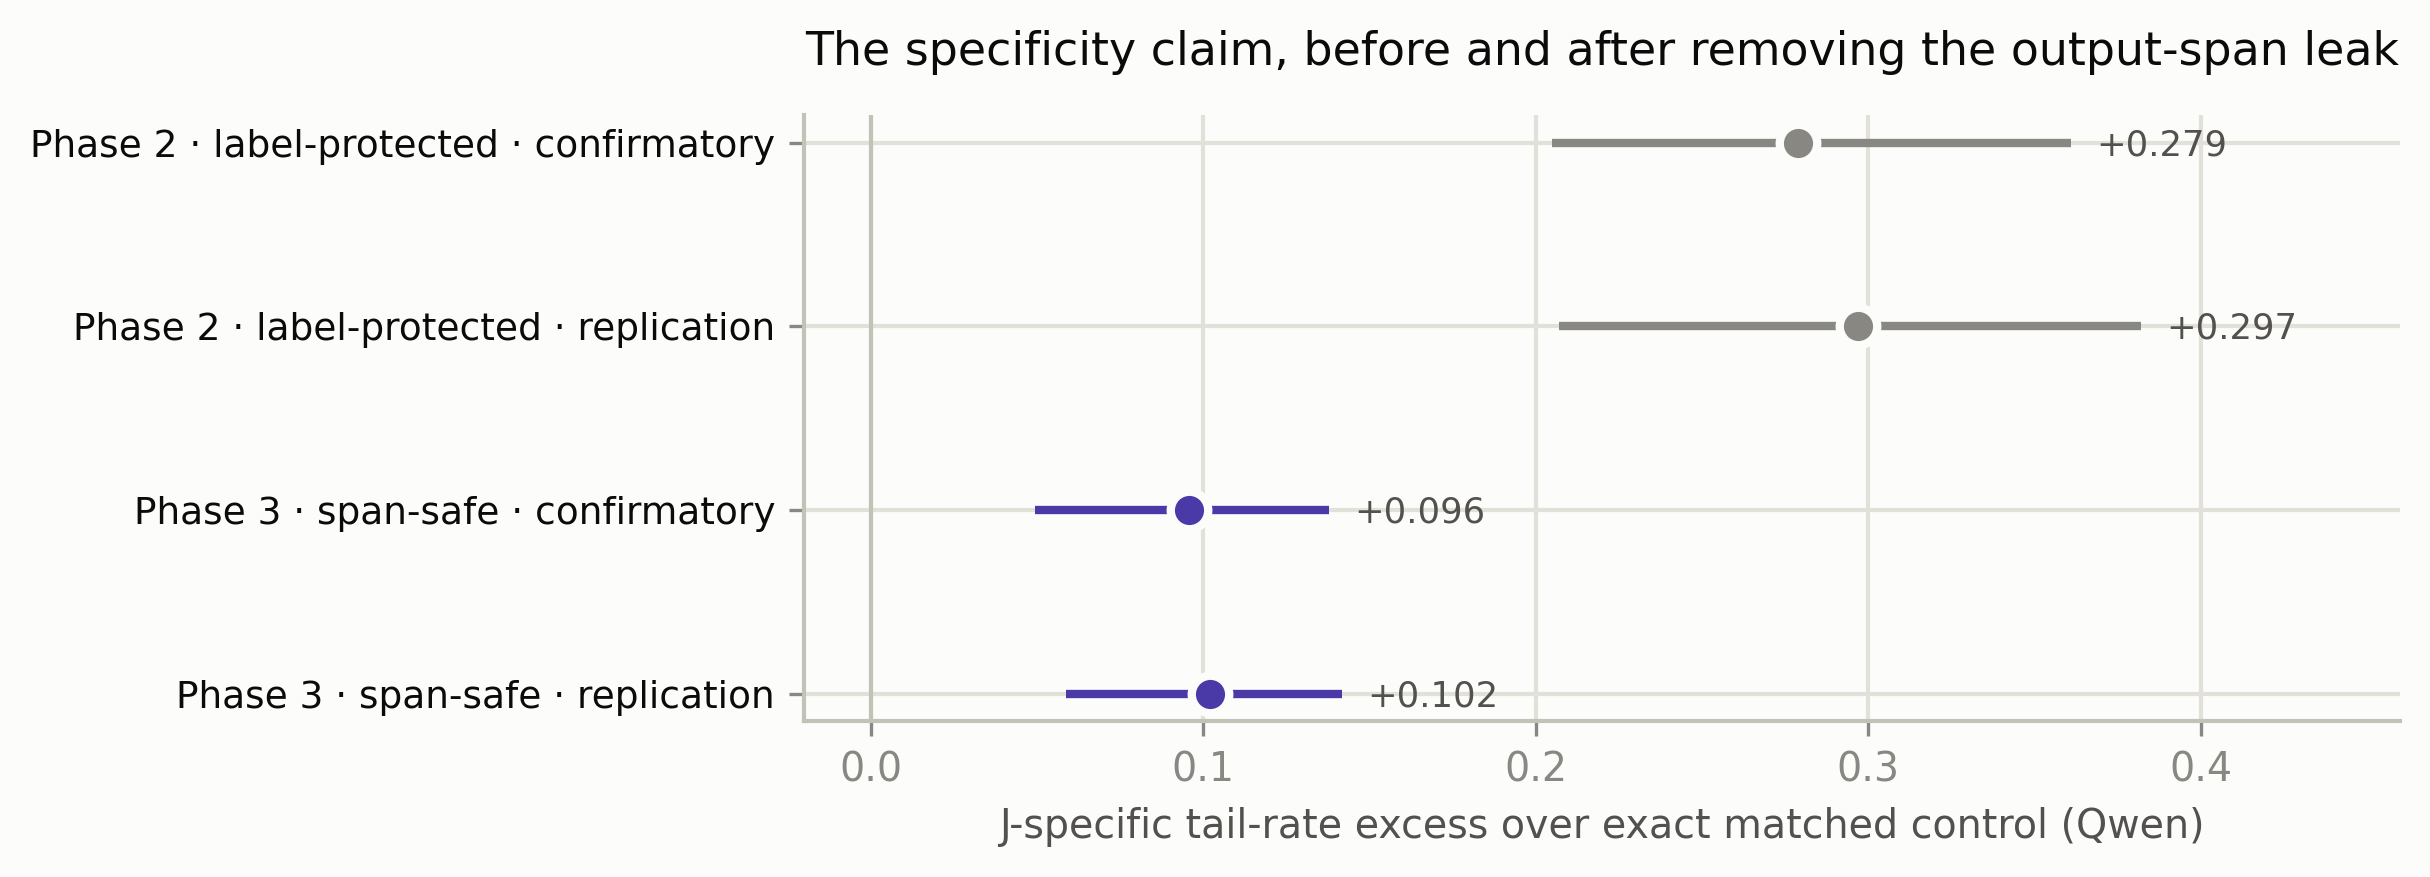
\includegraphics[width=0.97\textwidth]{figE_eras.png}
\caption{Qwen's specificity claim before and after output-span repair. The
large label-protected Phase 2 tail shrinks under span-safe protection but
survives and replicates in Phase 3. This is the confirmatory anchor against
which the OLMo lineage development result is interpreted.}
\label{fig:eras}
\end{figure}

\subsection{Qwen is a positive comparison, not merely a bigger OLMo}

Qwen differs from OLMo on several independent axes:
\begin{itemize}
  \item It has higher measured J-space capacity: roughly 5--6\% centered
  excess and occupancy 3--4 under the published lens, versus OLMo's roughly
  0.4--1.3\% and occupancy 2.
  \item Its span-safe heavy tail rejects at confirmatory tier ($+0.096$) and
  replicates on held-out families ($+0.102$)
  \eid{p3-inference-audit-v1,p3-replication-analysis-v1}.
  \item Label-protected and span-safe effects mostly rescale the same items
  ($r=0.75$), while on OLMo they reallocate damage ($r=0.20/0.29$).
  \item Qwen consumes a readable bridge route: true-bridge protection rescues,
  bridge-only lesion harms, and counterfactual substitution moves generation.
  OLMo Think does not show the same bridge mediation under the current assay.
\end{itemize}

\begin{figure}[H]
\centering
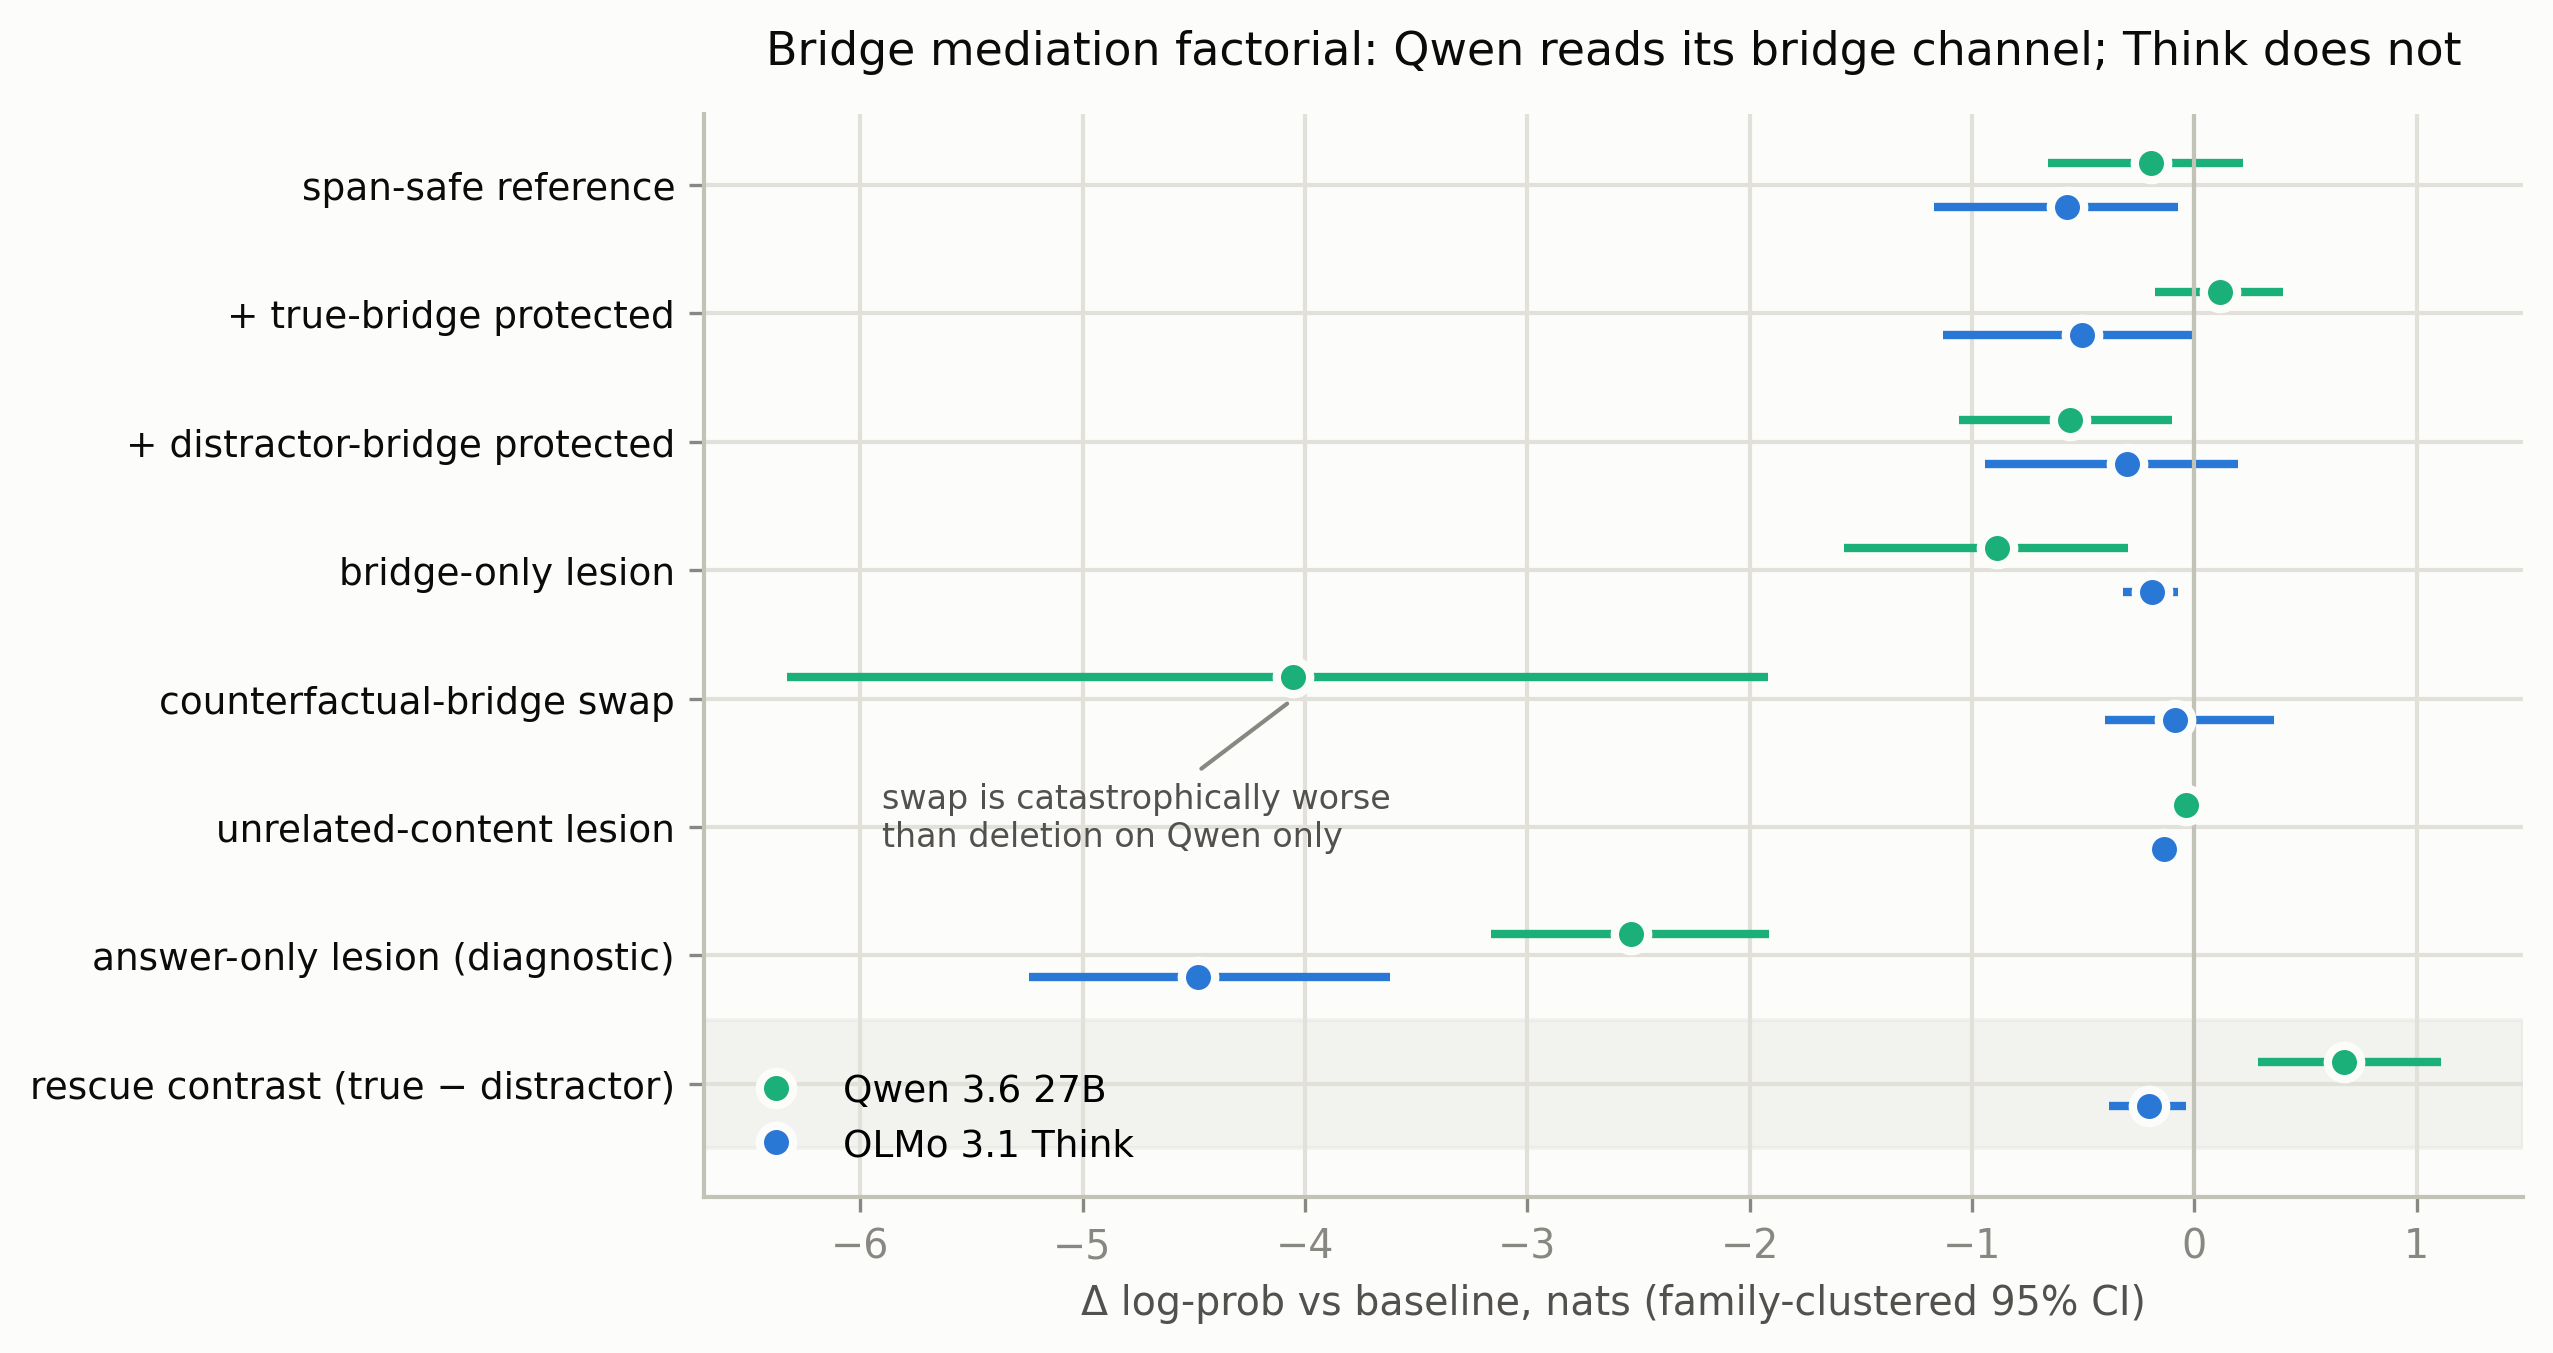
\includegraphics[width=0.96\textwidth]{figC_mediation_forest.png}
\caption{Development bridge mediation factorial. Qwen reads and follows the
bridge channel; OLMo-3.1 Think does not show the same route. The dramatic Qwen
swap is semantic, but Phase 4 still owes a bridge-versus-direct-answer-direction
contrast on an adequately powered untouched bank.}
\label{fig:bridge}
\end{figure}

Qwen therefore supplies a mechanistic contrast: a thicker, bridge-consumable
knowledge-access channel rather than the accessibility-organized OLMo regime.
It also supplies a methods warning. The Phase 4 same-corpus A120$\to$A250
lens comparison is structurally strong in the L20--L44 assay band, but selected
IDs and selected spans fail the frozen functional-stability thresholds. The
precommitted branch continues to A500
\eid{p4-qwen-lens-convergence-drawA-n120-n250-dev-v1,p4-qwen-multilens-functional-gate-a120-a250-published-dev-v1}.
Readout similarity and causal selection stability are not interchangeable.

\subsection{Gemma is not yet on the same scientific axis}

The supplied Gemma-4 31B pilot is shaped differently for a more fundamental
reason: the fixed linear transport premise appears to fail in the middle band.
The reported response becomes less homogeneous and less additive as delivered
perturbation scale grows, while the OLMo positive control approaches the
linear doubling rule. Independent corpus slices also disagree strongly at the
shallow edge. The appropriate current interpretation is not ``Gemma lacks a
workspace.'' It is ``the mid-band fixed J-lens is not licensed on this
checkpoint until an exact autograd-JVP versus finite-secant ladder closes the
transport gate.''

\begin{table}[H]
\centering\small
\begin{tabularx}{\textwidth}{@{}p{0.15\textwidth}p{0.18\textwidth}p{0.19\textwidth}X@{}}
\toprule
\textbf{System} & \textbf{Transport / coordinates} & \textbf{Measured causal organization} & \textbf{Most defensible current noun}\\
\midrule
Claude paper & J-lens method used to define a limited verbalizable subspace; this campaign has not rerun the transport gate on Claude & reported multi-step causal dissociation with fluency sparing & global-workspace interpretation in the source paper\\
Qwen 3.6 27B & usable published lens; small-lens convergence still functionally unsettled & replicated span-safe specific tail; bridge-consumable route & knowledge-access channel with bridge organization\\
OLMo 32B lineage & partial but useful transport; broad frame transfer; thin capacity & Think-path Bank-S dependence, accessibility organization, no Qwen-like bridge consumption & training-moderated verbalizable causal channel\\
Gemma 4 31B pilot & fixed mid-band linear transport not yet licensed & causal J-space assay cannot be interpreted on equal footing & methods boundary / nonlinear-transport case study\\
\bottomrule
\end{tabularx}
\caption{Cross-model comparison. Model differences are triangulation for the
OLMo training question, not a substitute for a causal training intervention.}
\label{tab:model-comparison}
\end{table}

Gemma's candidate causes include context-dependent tangent cancellation,
late basis conversion, attention routing transitions, repeated normalization
curvature, and gated-MLP interactions. None is yet established. The exact JVP
versus fp32 secant test, followed by layer and sublayer localization, is the
scientifically prior experiment.

%======================================================================
\section{Mechanistic hypotheses for the OLMo post-training effect}\label{sec:hypotheses}

These hypotheses are ordered by how directly they explain the lineage. Each
is explicitly falsifiable.

\begin{hypbox}{H1 -- Post-training recruits a conserved thin dictionary}
The broad J-readable coordinates already exist at base and survive into both
siblings. The Think recipe changes downstream consumption or persistence, not
capacity. This matches the common-frame trajectory, donor-lens transfer, flat
post-training capacity, and raw-arm decomposition.

\textbf{Against it:} aggregate frame robustness does not prove identical
subspaces or receivers; item-level frame shifts remain nontrivial.

\textbf{Decisive tests:} fit every OLMo checkpoint on one frozen corpus,
measure per-layer principal angles and top-$k$ selection overlap, then patch
Think activations or selected directions into Instruct under the common frame.
\end{hypbox}

\begin{hypbox}{H2 -- Think training makes prompt-supplied state substitute for internal state}
The positive Bank-S composed-minus-direct contrast may mean that a composed
prompt supplies an external scratchpad: the model relies less on its internal
J channel when the state is repeated or explicitly derivable in the prompt.
This would explain why direct Bank-S dependence is strongest at Think while
composed dependence is weaker.

\textbf{Against it:} the existing Bank-S templates confound composition,
redundancy, and derivation.

\textbf{Decisive test:} Bank W's fully crossed load $\times$
supplied/derived $\times$ once/redundant factorial. The primary cell is
internally derived, stated once; redundancy and supplied-state effects are
named interactions rather than explanations added after the fact.
\end{hypbox}

\begin{hypbox}{H3 -- Instruct routes retrieval through output-adjacent geometry}
The Instruct objective may optimize short direct answers, placing usable state
closer to output preparation. That is compatible with accessibility
organization, large label-arm damage on factual items, and near-zero Bank-S
span-safe dependence. Instruct may contain internal content while offering
less output-decoupled content for this assay to remove.

\textbf{Against it:} Phase 3 found the largest CI-clean span-safe content
residual on Instruct factual items; the effect is population-dependent.

\textbf{Decisive tests:} vary the protected-output span, separate fact recall
from in-context state, and localize receiver components under a fixed frame.
\end{hypbox}

\begin{hypbox}{H4 -- Accessibility, not workspace size, gates lesion cost}
Across the OLMo pair, damage concentrates on less output-locked answers;
Qwen reverses the sign. Think-path training may reorganize when retrieved
content becomes committed to the answer rather than how many concepts the
channel holds.

\textbf{Against it:} clean rank is already 1 for most lineage items, so the
coarse rank statistic may miss relevant confidence and margin structure.

\textbf{Decisive tests:} continuous answer-margin and entropy models on the
common-support cohort; matched-difficulty item construction; phase-resolved
interventions before and after answer commitment.
\end{hypbox}

\begin{hypbox}{H5 -- One unobserved post-training stage installs the effect}
The common-support data show an abrupt base$\to$3.0 Think change and no
resolved 3.0$\to$3.1 increment. The change may arise at a particular SFT,
preference, or reasoning stage rather than accumulate continuously.

\textbf{Against it:} released endpoints are too sparse to distinguish an
abrupt transition from a smooth change hidden inside the long interval.

\textbf{Decisive tests:} intermediate checkpoints, or a controlled
continuation from the base with the same evaluation frozen before training.
\end{hypbox}

%======================================================================
\section{General geometry lessons}\label{sec:geometry}

\subsection{Capacity is not causal privilege}

Within the OLMo post-trained trio, almost identical capacity coexists with
substantially different Bank-S dependence. Across models, Qwen's higher
capacity accompanies a cleaner bridge route, but three models are not a
moderator analysis. Capacity is best treated as one structural coordinate,
not as the explanation of causal organization.

\subsection{A stable readout can support changing downstream use}

A coordinate system can be conserved while the model changes which
activations enter it, which components read it, and whether alternative routes
compensate after ablation. This is analogous to retaining a shared interface
while replacing the implementation behind it. The OLMo evidence most directly
locates change downstream of broad coordinate availability.

\subsection{Output protection changes the population of damaged items}

On OLMo, label protection and true span protection damage different items.
Removing output-span leakage reallocates rather than merely shrinks the lesion.
That means post-training comparisons must name the protection geometry. A
single ``J-ablation effect'' can mix output-adjacent dose and internal-content
removal in model-dependent proportions.

\begin{figure}[H]
\centering
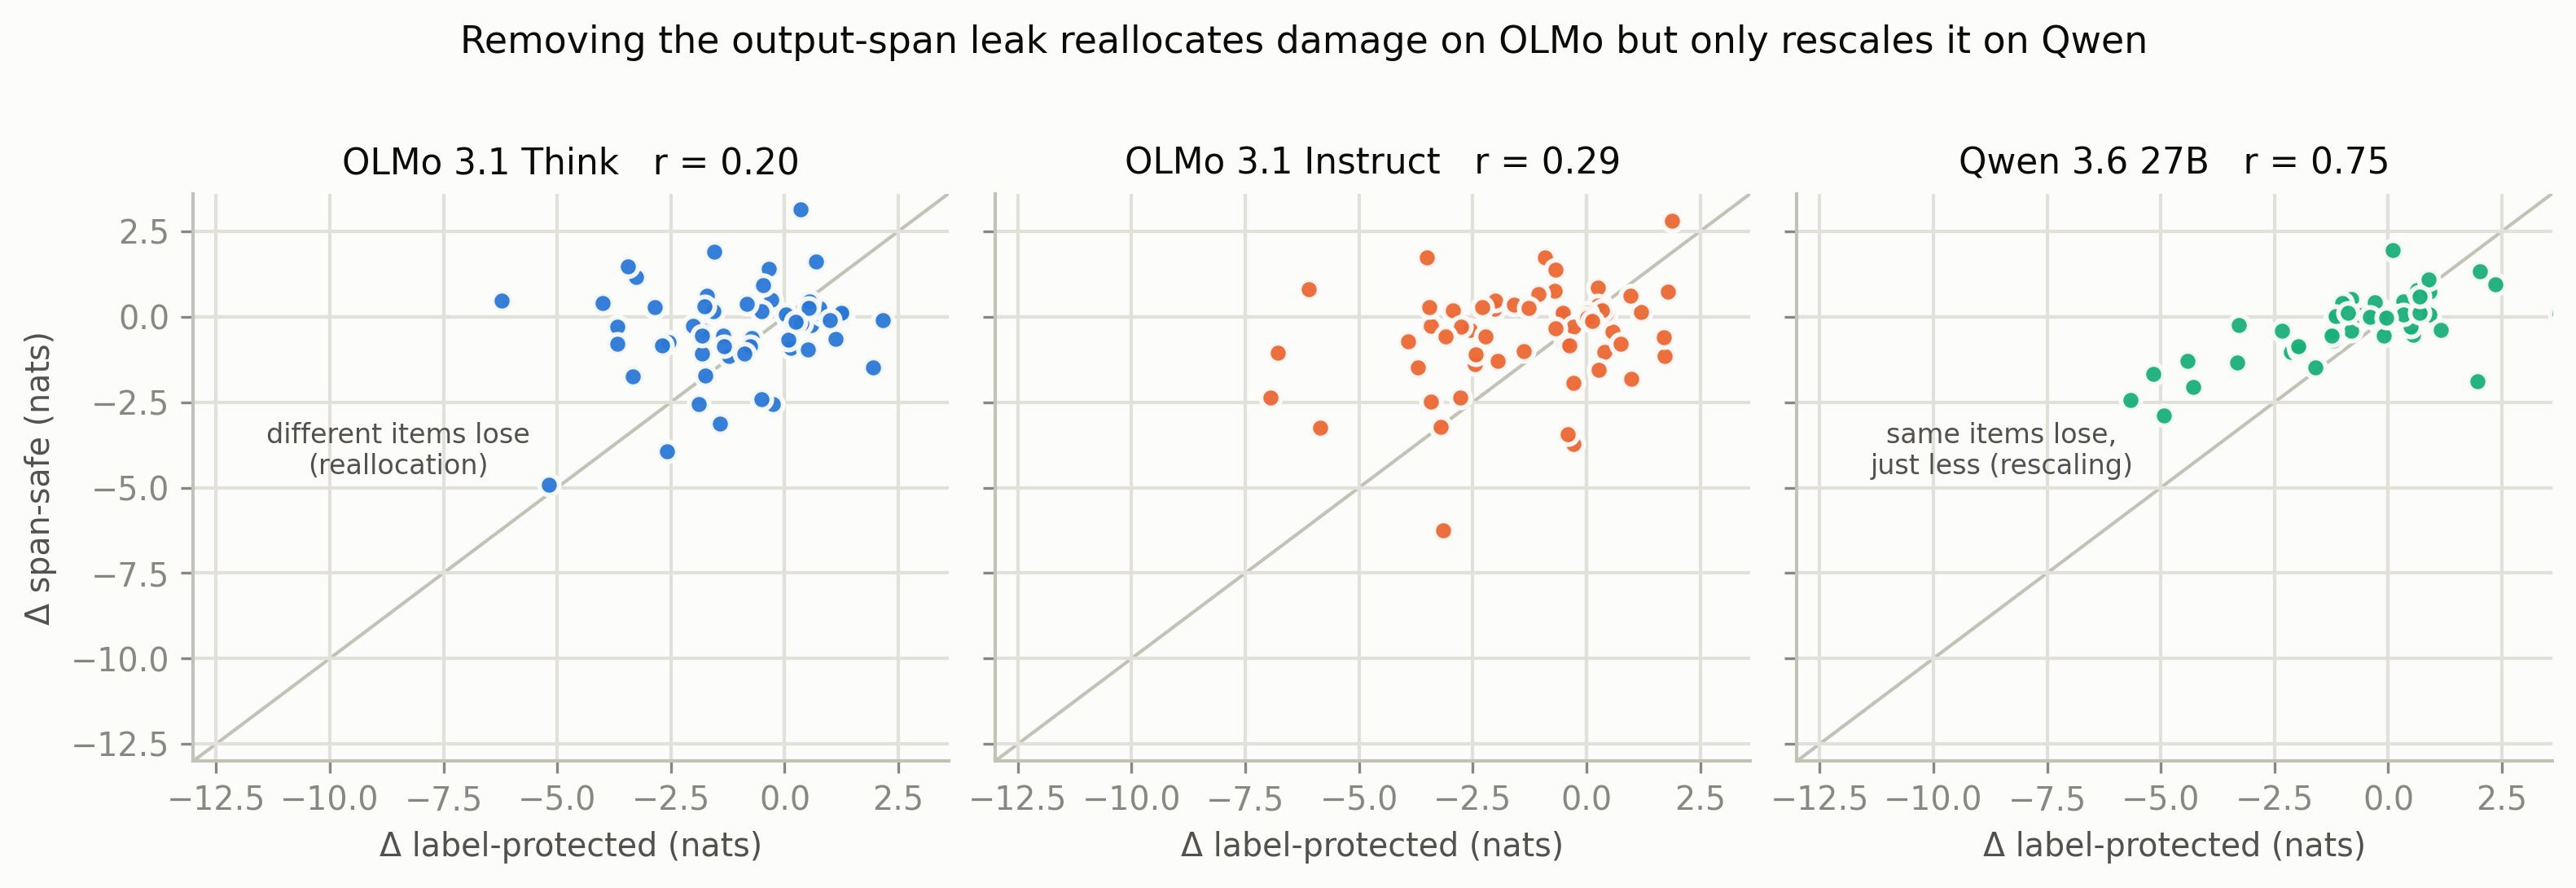
\includegraphics[width=0.97\textwidth]{figB_label_vs_spansafe.png}
\caption{Label-protected versus span-safe effects. On OLMo the low
correlations indicate reallocation; on Qwen the high correlation indicates
rescaling. Output protection is part of the scientific object, not a minor
implementation detail.}
\label{fig:reallocation}
\end{figure}

\subsection{Transport validity and workspace interpretation are separate gates}

OLMo can support a useful, if imperfect, fixed J coordinate through the
assay band. Gemma may not. A negative workspace result is uninterpretable
when the transport premise fails. Conversely, a readable lens is not by
itself a causal license. Every model family needs a separate finite-dose and
cross-context transport gate before it enters a shared J-space matrix.

%======================================================================
\section{Open questions and the next experiments}\label{sec:next}

\subsection{Highest-value OLMo experiments}

\begin{enumerate}
  \item \textbf{Run the Bank W capability and intervention gates on the OLMo
  pair first.} \emph{Resolved as gated out (\cref{sec:parallel}):} both OLMo
  endpoints pass individually, but the three-model intersection lands at
  16/24 families against the prospective 20 minimum, so the intervention
  factorial never opened \eid{ol-bank-w-capability-joint-dev-v1}. The
  externalization account stays unadjudicated; a successor bank needs a new
  prospective service protocol.

  \item \textbf{Measure base capacity with the identical estimator.}
  \emph{Done:} the symmetric O2 run includes base and returns
  \texttt{broadly\_conserved\_capacity\_recruitment\_consistent} ---
  occupancy difference exactly 0, centered excess $+0.015$pp
  \ci{-0.012}{+0.043} \eid{ol-capacity-joint-dev-v1}.

  \item \textbf{Build a same-corpus lens-geometry trajectory.} \emph{Done:}
  the provenance audit certified all six lenses same-recipe/same-corpus and
  the joint geometry run returned the dictionary-formation pattern
  (\cref{sec:parallel}; base$\to$3.0 mapped-row cosine 0.67 and selected-ID
  Jaccard 0.33 versus 1.0 for 3.0$\to$3.1)
  \eid{ol-lens-provenance-audit-v1,ol-geometry-joint-dev-v1}. Finite-dose
  per-checkpoint transport (H6) remains the missing validity leg.

  \item \textbf{Acquire intermediate post-training checkpoints or run a
  controlled continuation.} \emph{Upgraded to a concrete queue:} the official
  32B Think-SFT and Think-DPO artifacts are inventoried, semantically
  tokenizer-compatible, and eligible for a bounded two-cell stage wedge (H5,
  queued-not-started) \eid{ol-checkpoint-inventory-v2}.

  \item \textbf{Localize downstream receivers.} On the strongest Bank-S
  families, patch clean Think activations into ablated Think and into Instruct,
  then search attention/MLP receiver components with wrong-layer, unrelated,
  and dose-matched controls.

  \item \textbf{Resolve generation phase.} Teacher-forced log probability is
  the clean primary, but Think training is fundamentally about a generation
  policy. Add prefill-only, reasoning-only, and final-answer interventions with
  fixed parser and truncation rules.
\end{enumerate}

\subsection{Current Phase 4 blockers and why they matter}

\begin{itemize}
  \item \textbf{Qwen lens convergence:} A120$\to$A250 structure is strong,
  but selected-ID Jaccard and projector overlap fail frozen functional
  thresholds. The branch continues to A500. This blocks declaring a small
  Qwen lens canonical; it does not erase the published-lens Phase 3 results.
  \item \textbf{Qwen mode gate:} the first official thinking-on/off baseline
  failed because thinking-on truncated or failed to close on 7/20 families,
  leaving insufficient common support. A prospectively amended 2048-token gate
  is queued; no mode intervention claim exists yet.
  \item \textbf{Bank B bridge primary:} the verified 40-family candidate is
  dramatically underpowered for the proposed bridge-specific intersection-
  union endpoint. Reallocating the split cannot fix it. The design needs a new
  estimand or much larger bank, not a conveniently enlarged SESOI.
  \item \textbf{Phase 4 freeze:} the candidate preregistration remains
  unfrozen. No untouched confirmatory or replication outcome is licensed
  before protocol completion, independent review, PI sign-off, freeze commit,
  and tag.
\end{itemize}

\subsection{Gemma: the autopsy ran and terminated at a methods blocker}

The Gemma block did run as exactly the autopsy prescribed here (isolated
\texttt{jspace\_gemma} track, evidence prefix \texttt{gm-}). The exact-JVP
instrument passed goldens; the OLMo positive control passed all 14 frozen
criteria; Gemma Stage 1 then reported \texttt{local\_tangent\_mismatch} at
all five tested layers (L22--L52) --- but the run terminated at a failed
precommitted cross-backend parity gate (full-batch relative error 0.002458
against a $10^{-5}$ ceiling), so mechanism, curvature, heterogeneity,
late-band, and workspace interpretation are all unlicensed
\eid{gm-jvp-gemma-stage1-v1,gm-jvp-gemma-backend-parity-v1}. Stages G2--G8
were cancelled by the hard stop. The licensed sentence is methods-only; the
full story, figure, and claim ledger now live in the Gemma handout's
``The autopsy ran'' section. For this document the consequence is unchanged
but sharper: Gemma stays off the lineage's scientific axis until a repaired
backend-parity gate passes under a new evidence id.

%======================================================================
\section{Paper-facing conclusions and prohibited shortcuts}\label{sec:claims}

\begin{claimbox}[title={Recommended development-tier conclusion paragraph}]
Across four released checkpoints of the OLMo 32B lineage, span-safe J-specific
dependence on in-context Bank-S state is absent at the base model, appears by
the first observed Think checkpoint, persists at OLMo-3.1 Think, and is absent
at the OLMo-3.1 Instruct sibling. The pattern survives a frozen base-model
lens and exact common-support fact pairing, while measured J-space capacity is
conserved across all four checkpoints (occupancy difference exactly zero,
centered excess within $\pm0.25$-point equivalence margins) and the J-mapped
token dictionary reorganizes sharply in the same base$\to$Think interval
before freezing. These results support a training-moderated
causal-utilization account: post-training changes how --- and through which
token directions --- a thin verbalizable channel is recruited or routed,
rather than enlarging the measured channel. Because the checkpoints do not
isolate the post-training stage and all results use known development banks,
the evidence does not identify the Think objective as causal or establish
workspace formation; the planned Bank-W externalization factorial was gated
out at 16/20 common families and remains unresolved.
\end{claimbox}

\begin{table}[H]
\centering\small
\begin{tabularx}{\textwidth}{@{}X X@{}}
\toprule
\textbf{Allowed now} & \textbf{Not allowed now}\\
\midrule
The OLMo Bank-S dependence localizes to the observed Think path under the development assay. & Think training creates a global workspace.\\
The result survives two coordinate frames and common-support facts. & The J dictionaries are identical across checkpoints.\\
Measured capacity is conserved across all four checkpoints under the frozen estimator and margins, while causal utilization moves. & ``Capacity is unchanged'' stated without ``measured,'' the estimator, and its equivalence margin.\\
The mapped token dictionary reorganizes at base$\to$Think and then freezes; the siblings share a dictionary while differing in causal use. & The dictionaries are identical, or transport is valid, from structural geometry alone.\\
Instruct does not show the Think Bank-S organization on this population. & Instruct has no internal verbalizable channel.\\
Qwen and Gemma triangulate model-dependent organization and method validity. & Architecture alone explains Qwen, OLMo, or Gemma.\\
\bottomrule
\end{tabularx}
\caption{Claim discipline for the lineage section of the eventual paper.}
\end{table}

%======================================================================
\section{Data, evidence, and reproduction}\label{sec:repro}

\subsection{Evidence map}

\begin{table}[H]
\centering\small
\begin{tabularx}{\textwidth}{@{}p{0.24\textwidth}X@{}}
\toprule
\textbf{Purpose} & \textbf{Registered evidence}\\
\midrule
Capability gates & \path{p4-g5-bank-*-dev-v*} (four OLMo checkpoints)\\
Own-lens grids and analyses & \path{p4-lineage-grid-*-dev-v1}; \path{p4-lineage-analysis-*}\\
Frozen base-lens grids & \path{p4-lineage-grid-*-common-base-lens-dev-v*}\\
Paired frame analyses & \path{p4-lens-frame-analysis-*}\\
Trajectory synthesis & \path{p4-lineage-trajectory-analysis-olmo-dev-v1}\\
Common-support closure & \path{p4-lineage-common-cohort-analysis-olmo-dev-v1}\\
Capacity and transfer & \path{r2-occupancy-*-v2}; \path{a0-transfer-gate-olmo31instruct-v1}\\
Phase 3 cross-model context & \path{p3-inference-audit-v1}; \path{p3-span-audit-cross-model-v1}; \path{p3-bridge-mediation-*}\\
Current methods blockers & \path{p4-qwen-multilens-functional-gate-*}; \path{p4-bank-w-power-dev-v1}; \path{p4-bank-b-design-feasibility-dev-v1}; \path{p4-qwen-mode-gate-dev-v1}\\
Parallel-phase release (\cref{sec:parallel}) & \path{ol-bank-w-capability-*-dev-v1}; \path{ol-capacity-joint-dev-v1}; \path{ol-lens-provenance-audit-v1}; \path{ol-geometry-joint-dev-v1}; \path{ol-geometry-figures-dev-v1}; \path{ol-checkpoint-inventory-v2}; \path{ol-o5-feasibility-decision-v1}; \path{ol-independent-reconstruction-v1}; \path{ol-phase4-final-import-bundle-v1}\\
Gemma transport track & \path{gm-jvp-goldens-v1}; \path{gm-jvp-olmo-positive-control-v1}; \path{gm-jvp-gemma-stage1-v1}; \path{gm-jvp-gemma-backend-parity-v1}\\
\bottomrule
\end{tabularx}
\end{table}

The five \texttt{olf01--olf05} figures are registered outputs of
\path{ol-geometry-figures-dev-v1}, copied verbatim from the parallel-phase
run mirror (\path{interpretability/jspace_runs/olmo_lineage_20260801/}); the
package registry is
\path{interpretability/jspace_olmo_lineage/reports/evidence_events.jsonl},
and the release ledger is
\path{reports/OLMO_LINEAGE_CLAIMS_TABLE.md} in the same package.

\subsection{Regenerating the new synthesis figure}

The supplied script reads the registered trajectory CSV and replots its stored
point estimates and confidence limits. It does not recompute any bootstrap.
From a Phase 4 run root:

\begin{lstlisting}[basicstyle=\ttfamily\footnotesize,breaklines=true]
python olmo_lineage_synthesis_plots.py \
  --run-root /content/drive/MyDrive/interpret/special-lab-1/phase4_20260731 \
  --out-dir ./figures
\end{lstlisting}

The expected input is
\path{metrics/olmo-lineage-trajectory/trajectory_analysis/}
\path{p4-lineage-trajectory-analysis-olmo-dev-v1/}
\path{trajectory_table_olmo-lineage-trajectory.csv}.
A direct \texttt{--trajectory-csv} path is also accepted.

Existing \texttt{p4f*} figures remain products of their event-registered repo
producers. The attached \texttt{olmoL1--L4} figures are paper-local synthesis
plots built from registered trajectory, G5, lineage-analysis, and R2 outputs.

%======================================================================
\appendix
\section{Per-checkpoint panels}\label{app:panels}

These panels retain the full local context for each endpoint while the main
text carries only the synthesis figures.

\begin{figure}[H]
\centering

\includegraphics[width=0.86\textwidth]{p4f03_olmo3_base_development.png}
\caption{OLMo-3 32B base development point
\eid{p4-lineage-analysis-olmo3-base-dev-v1}.}
\end{figure}

\begin{figure}[H]
\centering
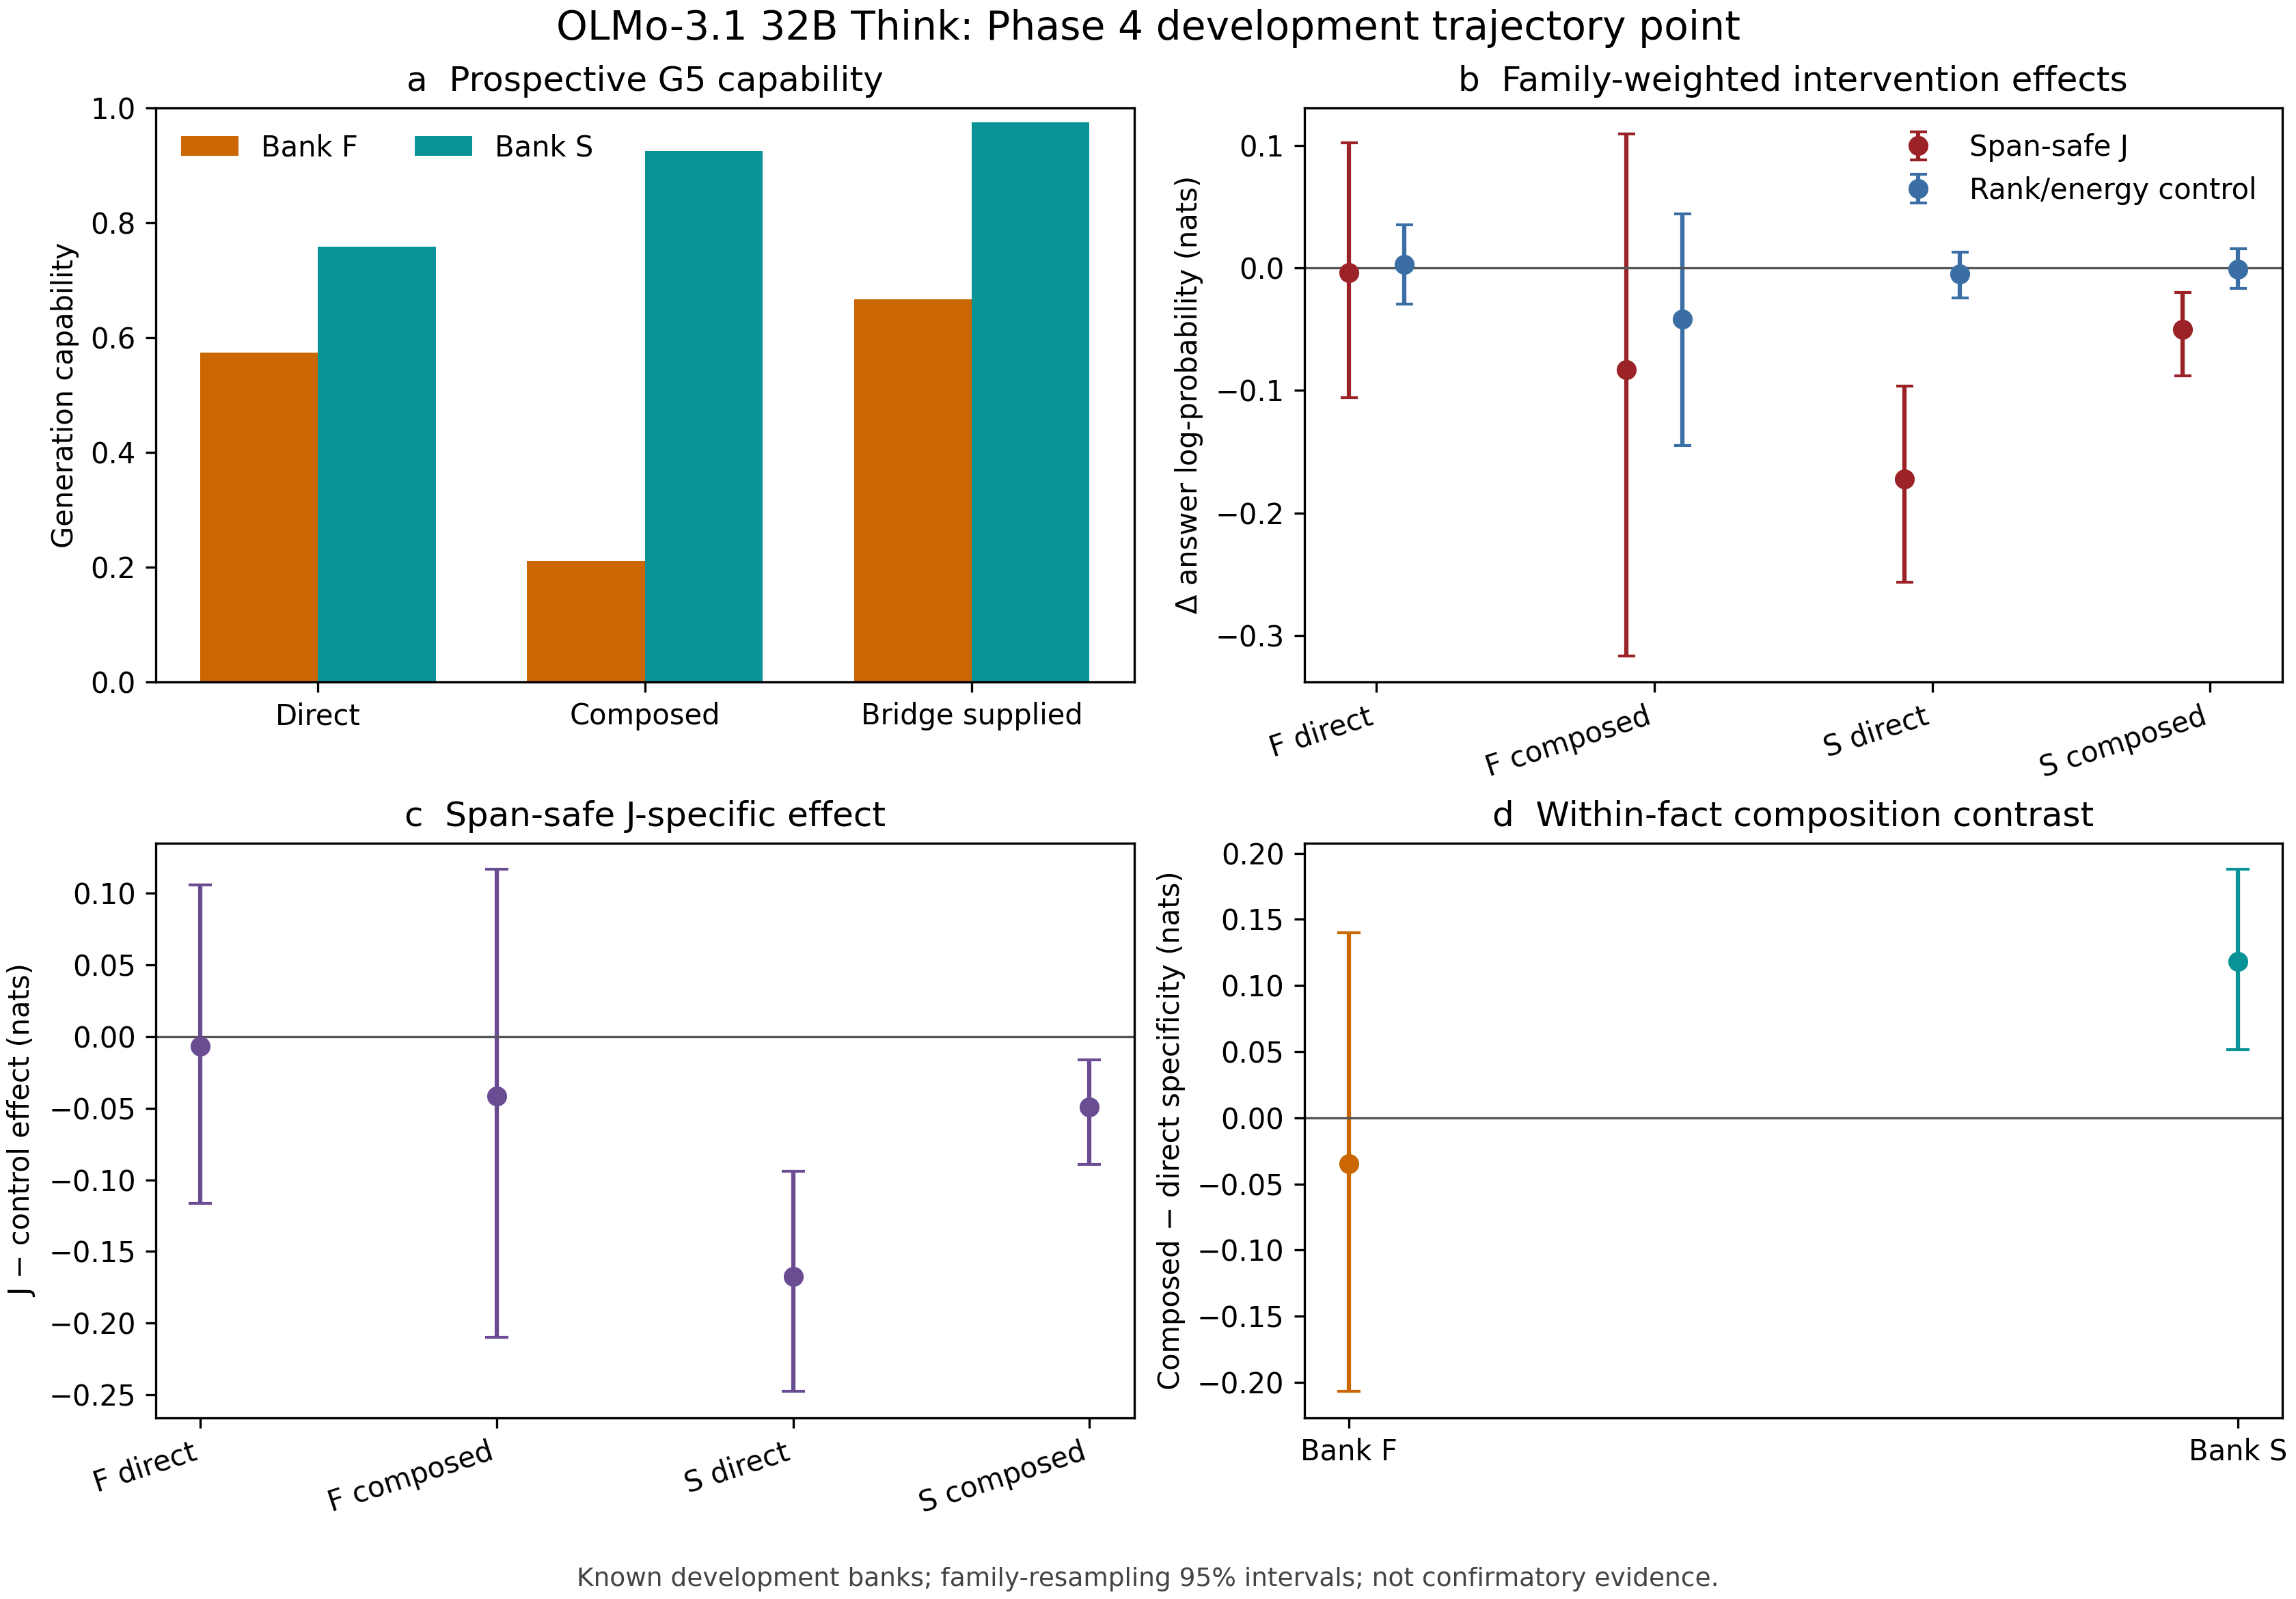
\includegraphics[width=0.86\textwidth]{p4f04_olmo31_think_development_v2.png}
\caption{OLMo-3.1 32B Think own-lens development point
\eid{p4-lineage-analysis-olmo31-think-dev-v2}.}
\end{figure}

\begin{figure}[H]
\centering
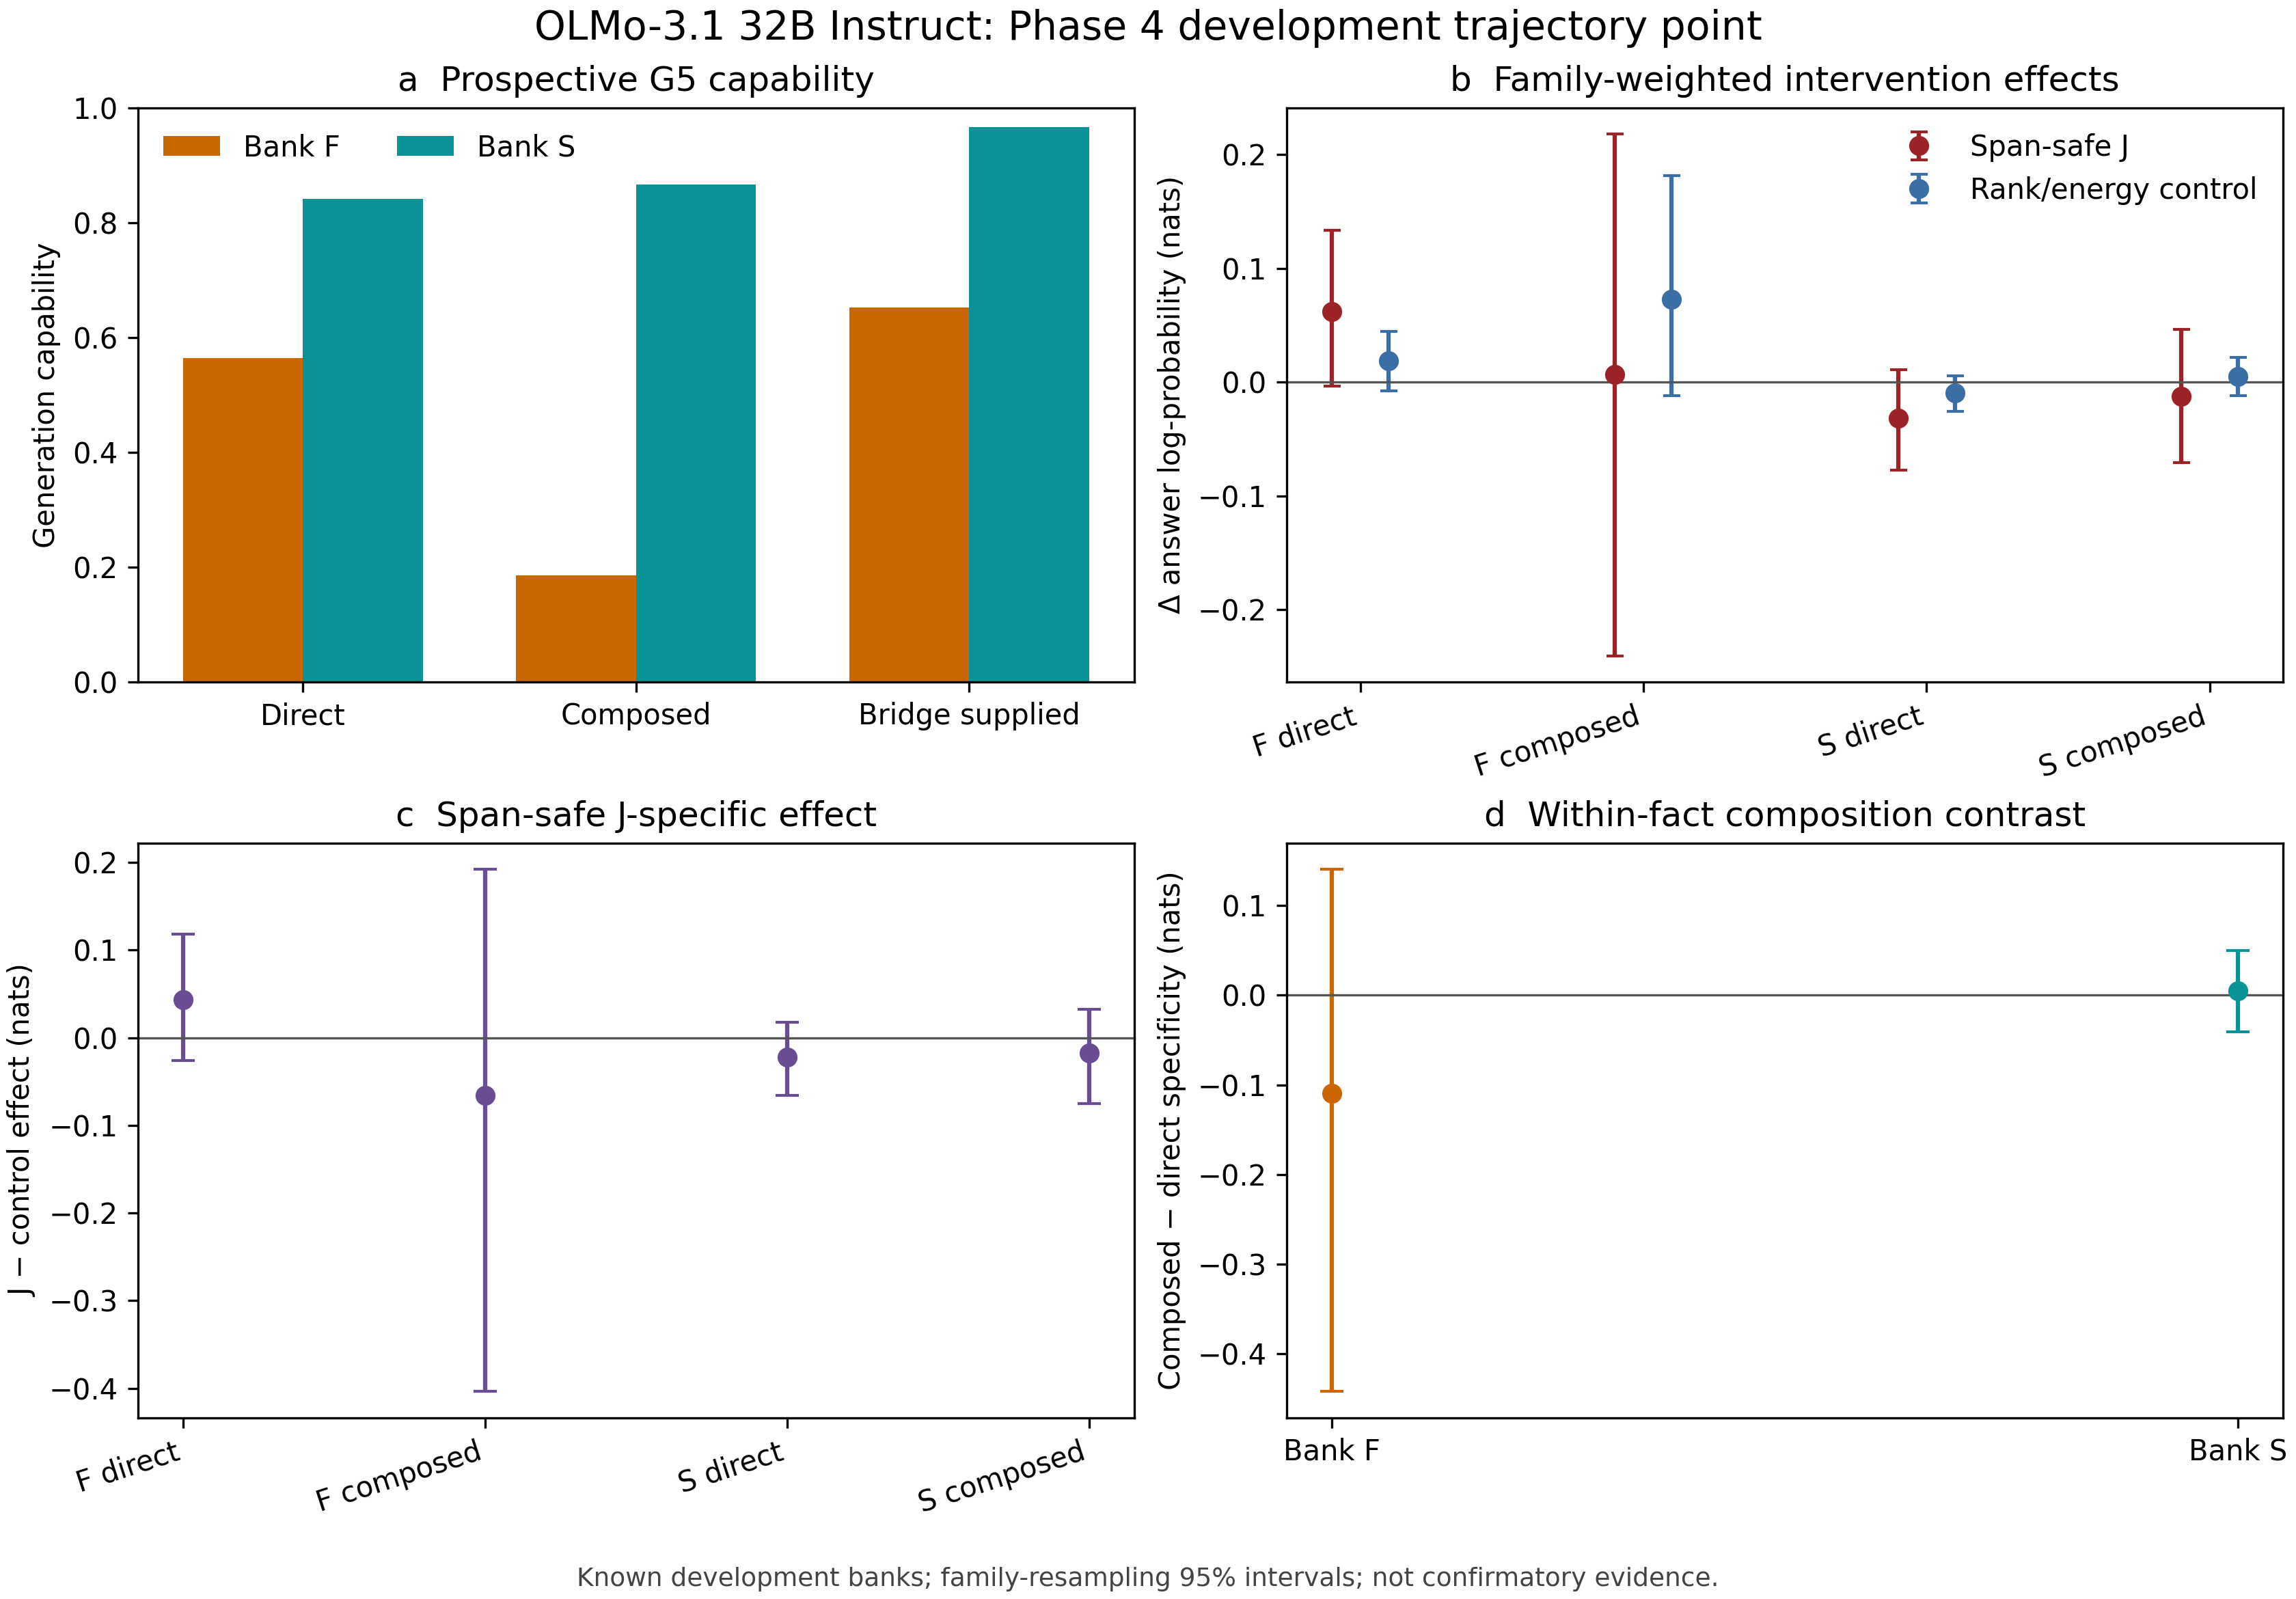
\includegraphics[width=0.86\textwidth]{p4f06_olmo31_instruct_development.png}
\caption{OLMo-3.1 32B Instruct own-lens development point
\eid{p4-lineage-analysis-olmo31-instruct-dev-v1}.}
\end{figure}

\section{Earlier-phase context}\label{app:earlier}

\begin{figure}[H]
\centering
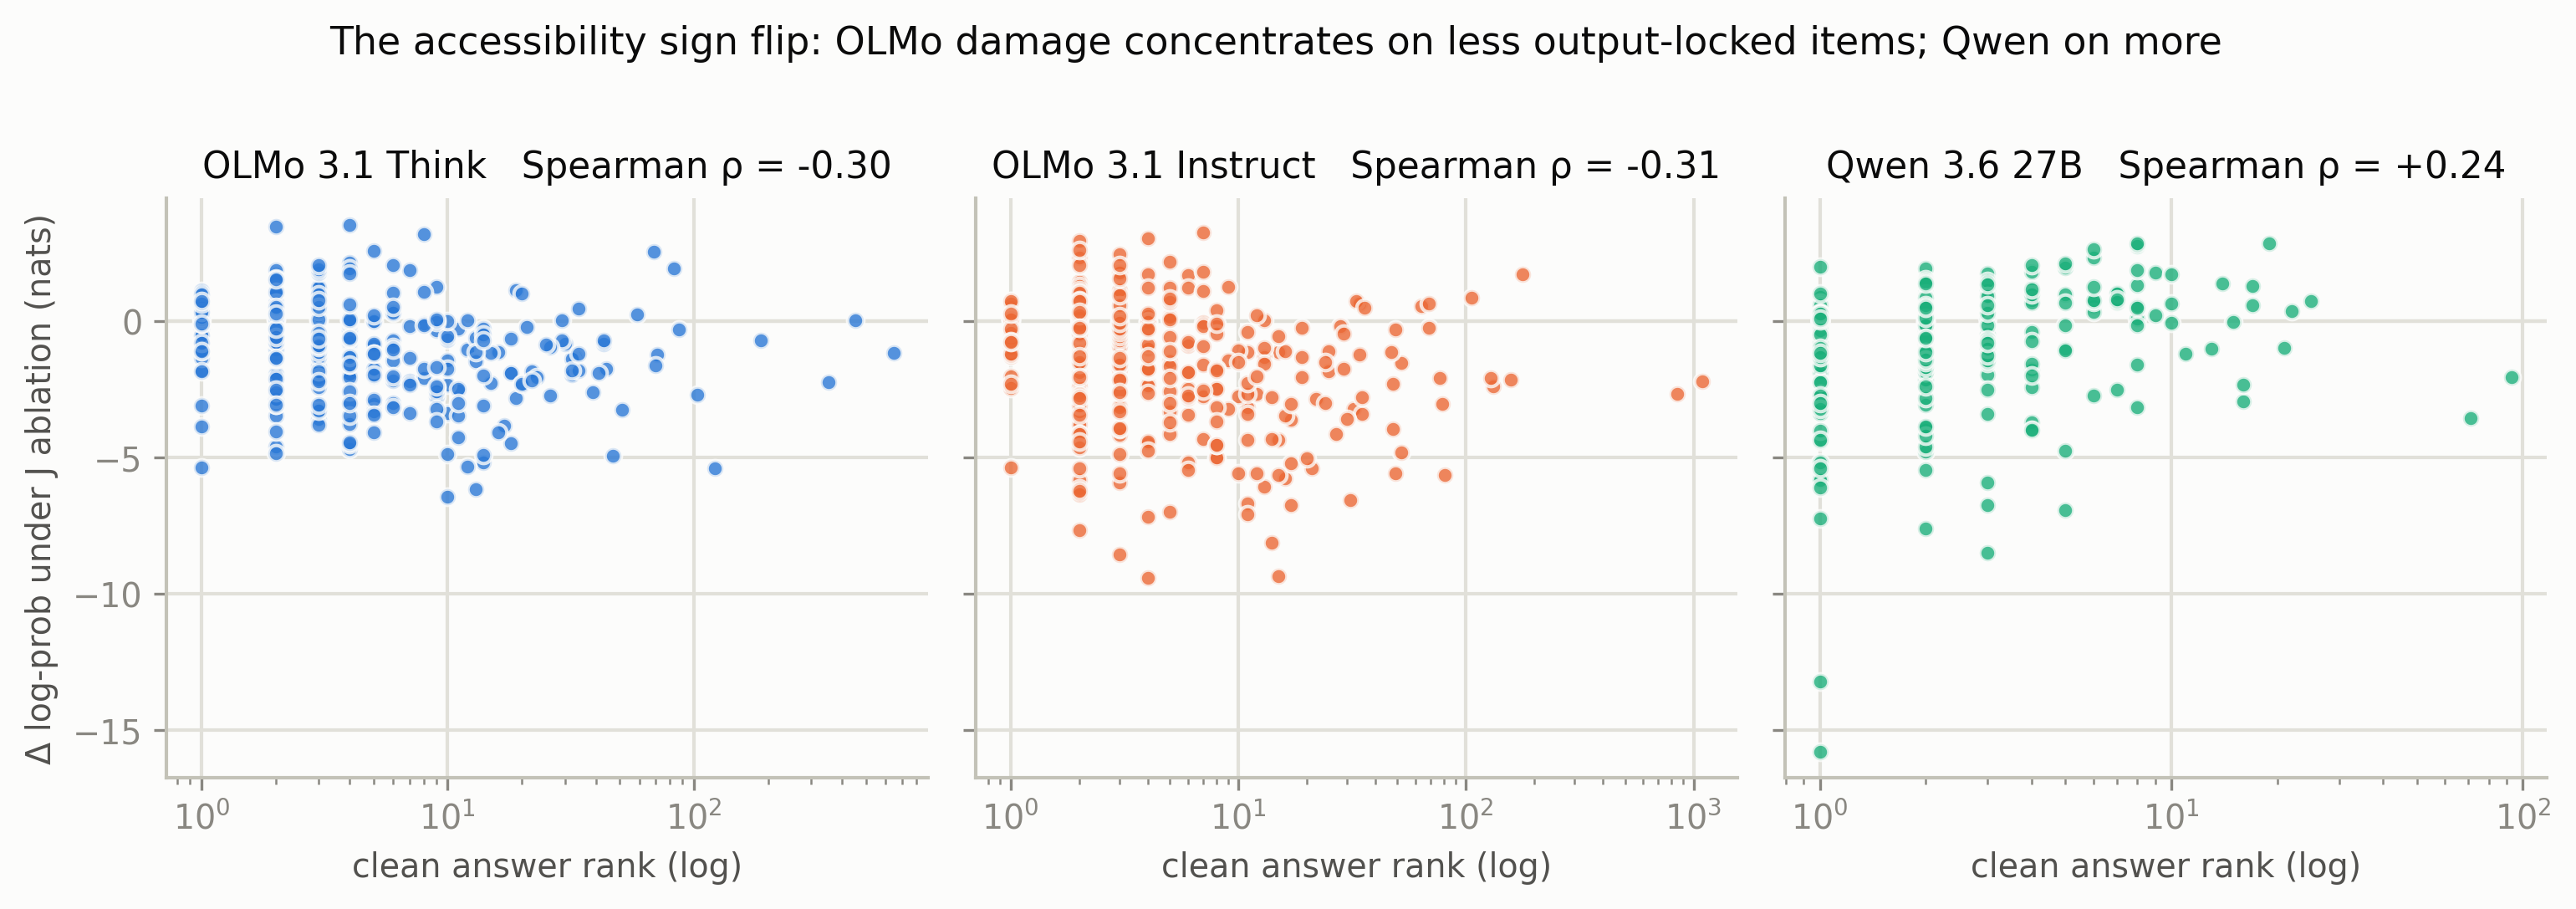
\includegraphics[width=0.97\textwidth]{figD_accessibility.png}
\caption{Phase 3 accessibility organization. OLMo damage concentrates on
less output-locked items, while Qwen has the opposite sign
\eid{p3-overlap-mining-v1}.}
\end{figure}

\begin{figure}[H]
\centering

\includegraphics[width=0.96\textwidth]{p2f4_r2_occupancy.png}
\caption{Earlier corrected capacity comparison. OLMo's occupancy is thin;
Qwen sits nearer the lower edge of the source paper's excess-variance range.
Later Phase 4 fit-size work adds a functional-convergence caveat to small-lens
comparisons.}
\end{figure}

\section{Revision note}

This rewrite removes the prior draft's meta-review from the main argument,
places the checkpoint panels in an appendix, defines three distinct meanings
of J-space formation, centers the capacity-versus-utilization dissociation,
adds the common-support closure and current Phase 4 methods boundaries, and
uses Qwen and Gemma as triangulation rather than as a flat model leaderboard.
No registered OLMo point estimate was changed.

\end{document}
